

\chapter{Calculus}\label{chapter:calculus}
\begin{figure}[H]
  \centering 
  \begin{tikzpicture}
    \begin{scope}[every node/.style={inner sep=0.5cm}, font=\ttfamily\scriptsize, anchor = east, rounded corners, line width = 0.4mm]
  \node[align=left, fill=sourceBackground, draw=sourceHighlight] (source-program) {\,\$(\textbf{do}$\, x \leftarrow \equote[\return{\texttt{0}}]$\\
  \,\quad \textbf{in} $(\lambda z. \return{z})(x))$};
  \node[align=left, fill=coreBackground, draw=coreHighlight] (core-program) at ($(source-program.east) + (6.4cm, 0cm)$){\textbf{tls}(\textbf{do}$\, x \leftarrow \return{\texttt{Ret}(\texttt{Nat}(\texttt{0}))}$ \\ 
  \quad\quad\textbf{in} $(\lambda z. \return{z})(x)$$)$};

  \node[align=left, fill=effBackground, draw=effHighlight] (normal-form) at ($(core-program.east) + (4cm, 0cm)$) {Ret$($Nat$(\texttt{0}))$\\ };
  \end{scope}

  \begin{scope}[every node/.style={font = \scriptsize}]
    \node[fill=sourceHighlight] (source-lang) at ($(source-program.south) + (0cm, 0cm)$ ) {\textcolor{white}\sourceLang{}};
    \node[fill=coreHighlight] (core-lang) at ($(core-program.south) + (0cm, 0cm)$ ) {\textcolor{white}\coreLang{}};
    \node[fill=effHighlight] (eff-lang) at ($(normal-form.south) + (0cm, 0cm)$ ) {\textcolor{white}\efflang{}};
  \end{scope}

  \begin{scope}[scale=8]
  \node[] (elaboration) at ($(source-program.east) + (0.095cm, -0.004cm)$) {\Huge$\leadsto$};
  \node[] (execution) at ($(core-program.east) + (0.095cm, 0.005cm)$) {\Huge$\rightarrow^{\text{\normalsize{$*$}}}$};
  \end{scope}

  \begin{scope}[every node/.style={font = \sffamily\tiny, anchor = south}]
  \node[] (elaboration-caption) at ($(elaboration) + (0cm, 0.3cm)$) {\textbf{Elaboration}};
  \node[align=center] (execution-caption) at ($(execution) + (0cm, 0.3cm)$) {\textbf{Compile-Time} \\ \textbf{Execution}};
  \end{scope}

  \end{tikzpicture}
  
  \caption{\calculusName{} is first elaborated into \coreLang{}, which is then executed \textbf{at compile-time} to obtain the AST of a run-time \efflang{} program.}%
  \label{fig:elaboration-then-execution}
\end{figure}

This thesis considers the interaction between homogenous, compile-time, two-stage \textbf{metaprogramming} (\Cpageref{section:metaprogramming-technical}), and deep, unnamed \textbf{effect handlers} with multi-shot continuations (\Cpageref{section:effects-technical}). This chapter describes a calculus, \calculusName{}, for studying said interaction.\ \calculusName{} has both metaprogramming and effect handlers. To the best of my knowledge, this is the first calculus in which both the generating and generated code may use effect handlers. However, \calculusName{} does not mediate the interaction between metaprogramming and effects: scope extrusion prevention is not a language feature. Rather, the aim is to extend \calculusName{} with various scope extrusion checks, and evaluate these checks in a comparative fashion. 

Programs written in \calculusName{} cannot be directly executed. Rather, following the style of \citet{xie-2023}, one must first elaborate (or compile) from \calculusName{} (the ``source'' language) to \coreLang{} (the ``core'' language).\, Programs written in \coreLang{} may then be executed, to obtain the AST of a run-time \efflang{} program. This process, which mirrors the approach by \citet{calcagno-2003}, is summarised in \Cref{fig:elaboration-then-execution}. Elaboration is useful, since it simplifies the operational semantics, and is a convenient mechanism for inserting dynamic checks (\Cref{chapter:scope-extrusion}). 

This chapter first introduces \sourceLang{} (\Cref{section:source-lang}), then \coreLang{} (\Cref{section:core-lang}). Following this, \Cref{section:elaboration} describes the elaboration from \sourceLang{} to \coreLang{}, and \Cref{section:metatheory} discusses the metatheoretic properties of \calculusName{}. 
% At a high-level, however, the names are suggestive: \sourceLang{} extends \efflang{} with quotation $\equote$ and splicing $\splice$, and \coreLang{} extends \efflang{} with AST constructors. 

\section{The Source Language: \texorpdfstring{\sourceLang{}}{Lambda-Op-Quote-Splice}}\label{section:source-lang}
\begin{figure}
\begin{source-desc}
  {\large \textbf{Syntax}} \\

  $\begin{array}{@{}llll}
    \textbf{Values} & v & ::= & \text{the natural lifting of \efflang{} values, with no term former for continuations}\\
    \textbf{Expressions} & e & ::= & \text{the natural lifting of \efflang{} expressions} \mid \equote \mid \splice \\
    \textbf{Handlers} & h & ::= & \text{the natural lifting of \efflang{} handlers}
  \end{array}$
\end{source-desc}
\caption{\sourceLang{} syntax. The syntax is broadly the same as \efflang{}, except with the addition of quotes and splices, and the removal of the continuation term former $\kappa x.e$.}
\label{fig:source-syntax}
\end{figure}
\sourceLang{} extends \efflang{} with quotes and splices. Additionally, the continuation term former $\kappa x. e$ is removed, since it cannot be written explicitly in \efflang{}, only generated during reduction -- but \sourceLang{} has no reduction semantics. Recall that \efflang{} divides terms into three syntactic categories: values ($v$), computations ($c$), and handlers ($h$).\ \sourceLang{} is similar, dividing terms into values ($v$), expressions ($e$), and handlers ($h$) (\Cref{fig:source-syntax}).

Only expressions can be quoted (values cannot be): thus, quotes must generate run-time computations. For example, $\equote[\texttt{1}]$ is not valid syntax, instead, one must write $\equote[\return{\texttt{1}}]$. Similarly, $\equote[\return{\texttt{1}}]$ is an expression, not a value, so one must write: 
\[\bind{a}{\equote[\return{\texttt{1}}]}{\op{a}}\]
rather than $\op{\, \equote[\return{\texttt{1}}] \,}$. However, I will abuse notation and write $\op{\equote[\texttt{1}]}$ in place of $\bind{a}{\equote[\return{\texttt{1}}]}{\op{a}}$.

\subsection{Type System}\label{subsection:sourcelang-type-system}
\begin{figure}
  \begin{source-desc}
    $\begin{array}{lllr}
    {\textbf{\large {Effects Row}}}\\\\
    \textbf{Run-Time} & \xi ::= \emptyset \mid \xi \cup \{ \textsf{op}_i^{0}\} \\
    \textbf{Compile-Time} & \Delta ::= \emptyset \mid \Delta \cup \{ \textsf{op}_i^{-1}\} \\\\
    \end{array}$

\vspace{5mm}
  $\begin{array}{lllr}
    {\textbf{\large {Types}}}\\\\ \vspace{0.4mm}
    \textbf{Level 0} & \text{Values} & S^0, T^0 ::= \mathbb{N}^0 & \text{\footnotesize{naturals}} \\ \vspace{0.4mm}
    && \quad\quad\quad\,\,\,\; \mid {(\functionType[\xi]{S^0}{T^0})}^{0} & \text{\footnotesize{functions}} \\ \vspace{0.4mm}
    && \quad\quad\quad\,\,\,\; \mid {(\continuationType[\xi]{S^0}{T^0})}^{0} & \text{\footnotesize{continuations}} \\\vspace{0.4mm}
    & \text{Computations} & T^0 \, ! \, \xi \\\vspace{0.4mm}
    && \mid T^0 \, ! \, \Delta \\\vspace{0.4mm}
     && \mid T^0 \, ! \,  \Delta;\xi & \\\vspace{0.8mm}
    & \text{Handlers} & (\handlerType{S^0 \, ! \, \xi_1}{T^0 \, ! \, \xi_2})^0\, !\, \Delta\\ \\ 

    \textbf{Level $-$1} & \text{Values} & S^{-1}, T^{-1} ::= \mathbb{N}^{-1} & \text{\footnotesize{naturals}} \\ \vspace{0.4mm}
    && \quad\quad\quad\quad\quad \mid {(\functionType{S}{T})}^{-1} & \text{\footnotesize{functions}} \\\vspace{0.4mm}
    && \quad\quad\quad\quad\quad \mid {(\continuationType{S}{T})}^{-1} & \text{\footnotesize{continuations}} \\\vspace{0.4mm}
    && \quad\quad\quad\quad\quad \mid {\textsf{Code}({T^{0} \, ! \, \xi})}^{-1} & \text{\footnotesize{run-time code}} \\\vspace{0.8mm}
    & \text{Computations} & T^{-1} \, ! \, \Delta \\\vspace{0.8mm}
    & \text{Handlers} & (\handlerType{S^{-1} \, ! \, \Delta_1}{T^{-1} \, ! \, \Delta_2})^{-1}
  \end{array}$
  \end{source-desc}
  \caption{\sourceLang{} types. Types are stratified into two levels, $0$ and $-1$. Similarly, effects are stratified into two levels, $\xi$ (run-time) and $\Delta$ (compile-time). The \textsf{Code} type allows compile-time programs to manipulate ASTs of run-time code.}
  \label{fig:source-types}
\end{figure}

The \sourceLang{} types are summarised in \Cref{fig:source-types}. There are three important details: types are stratified into two levels ($-1$ for compile-time and $0$ for run-time), effect rows are similarly stratified, and run-time code is made available at compile-time via a \textsf{Code} type.

First, \textbf{types are stratified into two levels, $T^0$ (run-time), and $T^{-1}$ (compile-time)}.

  To motivate this stratification, consider the type of the number \texttt{3} in \sourceLang{}. Perhaps surprisingly, the type of \texttt{3} is not $\mathbb{N}$. Since \sourceLang{} is a two-stage system, it carefully disambiguates between run-time naturals and compile-time naturals, since these are not interchangeable. For example, the following program should \textbf{not} be well-typed, since \texttt{3} is a compile-time natural, whereas $x$ is a run-time natural: 
  \[\lambda x: \mathbb{N}. \; \$(\texttt{3} + x)\]
  However, removing the splice makes the program well-typed:
  \[\lambda x: \mathbb{N}. \; \texttt{3} + x\]
  As is conventional for multi-staged languages, \sourceLang{} introduces integer levels to enforce separation between compile-time and run-time naturals. While the precise notion of level is slightly more involved (\Cref{dfn:level}), for \sourceLang{}, it is sufficient to think of level $0$ as run-time (so $\mathbb{N}^0$ is a run-time natural), and $-1$ as compile-time. Naturals can be annotated with levels, hence, the ill-typed example becomes:
  \[\lambda x: \mathbb{N}^0. \; \$(\textcolor{comment}{(\textcolor{black}{\texttt{3}}:\mathbb{N}^{-1})} + \textcolor{comment}{(\textcolor{black}{x}:\mathbb{N}^{0})})\]
  and the well-typed example becomes (note that, like naturals, the $+$ operator can be annotated with a level): 
  \[\lambda x: \mathbb{N}^0. \; \textcolor{comment}{(\textcolor{black}{\texttt{3}}:\mathbb{N}^{0})} + \textcolor{comment}{(\textcolor{black}{x}:\mathbb{N}^{0})}\]
  More precisely, levels are defined as follows:

  \begin{definition}[Level]{sourceHighlight}\label[definition]{dfn:level}
    The level of an expression $e$ is calculated by subtracting the number of surrounding splices from the number of surrounding quotations.
  \end{definition}

  The definition of level generalises to multi-stage languages, where negative levels ($-1, -2, \ldots$) represent compile-time and non-negative levels ($0, 1, \ldots$) represent run-time \footnote{Many existing languages only consider compile-time \textbf{or} run-time metaprogramming, not both, and will thus have either non-positive or non-negative levels.}. In a multi-stage language, separation is even more granular: for example, level $1$ and level $0$ run-time naturals are distinguished. However, since \sourceLang{} is a two-stage language, it is sufficient to consider only levels $0$ and $-1$. \Cref{dfn:level}, and the examples above, further imply that the ``default'' level, in the absence of quotes and splices, is level $0$. Intuitively, in the absence of quotes and splices, the programmer is ignoring metaprogramming facilities, and writing a run-time program. 


  It is impossible, without further information, to assign a type to \textit{program fragments}, like \texttt{3}. Without knowledge of the wider context, it is impossible to know which level the program fragment is at: in the ill-typed example, \texttt{3} occurs under a splice, but no quotes, so it occurs at level $-1$ and has type $\mathbb{N}^{-1}$. In contrast, in the well-typed example, \texttt{3} occurs at level $0$ and has type $\mathbb{N}^0$. Unless otherwise stated, I always assume program fragments occur at level $0$.

  Second, \textbf{effect rows are stratified into $\xi$ (run-time) and $\Delta$ (compile-time)}.\\
  The following example prints \texttt{1} at compile-time, and \texttt{2} at run-time. Further, it reads an integer at run-time.
\[\splice[{(\textbf{\texttt{print}}(\texttt{1}); \equote[\textbf{\texttt{print}}(\texttt{2}); \textbf{\texttt{readInt}}()])}]\]
Hence, $\Delta = \{ \textbf{\texttt{print}} \}$ and $\xi = \{ \textbf{\texttt{print}}, \textbf{\texttt{readInt}} \}$. Disambiguating run-time and compile-time effects stratifies types. Unlike in \efflang{}, where a term is either of value or computation type, in \sourceLang{}, the stratification of types is thus more granular:
\begin{enumerate}[leftmargin=5.8\parindent]
  \item[$T^0 \quad\quad\,\,$] Compile-time value, run-time value (value types) \\
  \textit{Example}: The type of $x$ in $\lambda x. \return{x}$
  \item[$T^0 \, ! \, \xi \quad\;$] Compile-time value, run-time computation  \\
  \textit{Example}: The type of $x$ in $\splice[(\bind{x}{\equote[\return{\texttt{1}}]}{\return{x}})]$
  \item[$T^0 \, ! \, \Delta \quad$] Compile-time computation, run-time value \\
  \textit{Example}: $\lambda x. \return{x}$ 
  \item[$T^0 \, ! \, \Delta; \xi$] Compile and run-time computation \\
  \textit{Example}: $\splice[(\bind{x}{\equote[\return{\texttt{1}}]}{\return{x}})]$
\end{enumerate}
Further, the relationship between syntax and types is more complicated than in \efflang{}. For example, level $0$ \sourceLang{} values ($v$) do not have value type ($T^0$). Rather, since level $0$ values are elaborated into compile-time computations  that produce ASTs of run-time values, they have computation type $\effectType{T^{0}}$ (\Cref{table:typing-judgements}). As the stratification is subtle, it is best revisited after covering the typing rules (\Cref{subsection:sourcelang-type-system}), core language (\Cref{section:core-lang}), and elaboration (\Cref{section:elaboration}).
% As a result of the type system, we never encounter $T^0 \, ! \, \Delta$ (compile-time computations that are run-time values).

Third, \textbf{there is a level $-1$ \textsf{Code} type, representing run-time ASTs}.\\ 
  Stratifying types ensures that run-time (resp.\ compile-time) terms only interact with run-time (compile-time) terms. However, to enable metaprogramming, run-time terms should be available at compile-time as ASTs. This is exactly the role of the \textsf{Code} type, thus allowing level $-1$ programs to manipulate ASTs of level $0$ terms.
% Note that if we had a multi-level system, then there would be a \texttt{Code} type at level $0$, representing the ASTs of level $1$ terms. The asymmetry arises from the restriction to two levels. 

Putting it all together, we can now interpret complex \sourceLang{} types, like the following:
\begin{center}
\begin{tikzpicture}

  \begin{scope}[local bounding box=group 1]
  \node[text width=\linewidth, align = center] (example) at (0, 0) {$(\functionType[]{{\textsf{Code}(\mathbb{N}^0 ! \{ \texttt{print} \})}^{-1}}{\textsf{Code}(\mathbb{N}^0 \, ! \, \{ \texttt{print}, \texttt{readInt} \})^{-1}})^{-1}$};
  '\end{scope}

  \node[align=center, font=\footnotesize](effects) at (-1.1cm,0.3cm){$\{ \texttt{get} \}$};

  \begin{scope}[on background layer, font=\scriptsize\bfseries, text=comment, align=left]
    \draw[draw=comment, line width = 0.3mm] ($(example.north east) + (-3.1cm, 0.6cm)$) circle[radius=1.4mm] node (annote-1) {\tiny{1}};
    \node[anchor = east, align=right] (annote-1-text) at ($(annote-1.west) + (0.1cm, -0.15cm)$) {Compile-time \\function} ;
    \draw[draw=comment, line width =0.3mm] ($(example.north east) + (-2.6cm, 0cm)$) |- (annote-1.east);

    \draw[draw=comment, line width = 0.3mm] ($(effects.north) + (-0.5cm, 0.4cm)$) circle[radius=1.4mm] node (annote-2) {\tiny{2}};
    \node[anchor = east, align=right] (annote-2-text) at ($(annote-2.west) + (0.1cm, -0.15cm)$) {Compile-time \\effects} ;
    \draw[draw=comment, line width =0.3mm] (effects.north) |- (annote-2.east);

    \draw[draw=comment, line width = 0.3mm] ($(example.south west) + (3.4cm, -0.4cm)$) circle[radius=1.4mm] node (annote-3) {\tiny{3}};
    \node[anchor = north west, align=left] (annote-3-text) at ($(annote-3.east) + (-0.1cm, 0.27cm)$) {Input: AST of a run-time \\ computation of type $\mathbb{N} \, ! \, \{\texttt{print}\}$} ;
    \draw[draw=comment, line width =0.3mm] ($(example.south west) + (2.9cm, 0cm)$) |- (annote-3.west);

    \draw[draw=comment, line width = 0.3mm] ($(example.south east) + (-7.5cm, -0.4cm)$) circle[radius=1.4mm] node (annote-4) {\tiny{4}};
    \node[anchor = north west, align=left] (annote-4-text) at ($(annote-4.east) + (-0.1cm, 0.27cm)$) {Output: AST of a run-time \\ computation of type $\mathbb{N} \, ! \, \{\texttt{print},\texttt{readInt}\}$} ;
    \draw[draw=comment, line width =0.3mm]  ($(example.south east) + (-8cm, 0cm)$) |- (annote-4.west);
  \end{scope}

\end{tikzpicture}


\end{center}
% Reading from the outside-in:
% \begin{enumerate}
%   \item This is a level $-1$, or compile-time function
%   \item The function has (suspended) compile-time effect \texttt{get} 
%   \item The function expects an AST of some run-time computation with type with type $\mathbb{N} \, ! \, \{\texttt{print}\}$
%   \item The function returns an AST of some run-time computation with type $\mathbb{N} \, ! \, \{\texttt{print},\texttt{readInt}\}$
% \end{enumerate}

\newcommand{\compilemode}{\textbf{\textsf{\textcolor{compile}{c}}}}
\newcommand{\splicemode}{\textbf{\textsf{\textcolor{splice}{s}}}}
\newcommand{\quotemode}{\textbf{\textsf{\textcolor{quote}{q}}}}
\subsubsection{Typing Judgements}
\begin{table}[H]
  \newcommand\T{\rule{0pt}{2.6ex}}       % Top strut
\newcommand\B{\rule[-1.2ex]{0pt}{0pt}} % Bottom strut
  \centering
  \begin{tabular}{l|l|l|l}
    & \textbf{Value } ($v$) & \textbf{Expression} ($e$) & \textbf{Handler} ($h$) \B \\ \hline 
    \textbf{Compile} (\compilemode{}) & $\Gamma \vdash^{0}_{\compilemode{}} v: \effectType{T^{0}}$ & $\Gamma \vdash^{0}_{\compilemode{}} e: \effectType[\Delta ; \xi ]{T^{0}}$ & $\Gamma \vdash^{0}_{\compilemode{}} h: (\handlerType{\effectType[\xi_1]{S^0}}{\effectType[\xi_2]{T^{0}}})^{0} \, ! \, \Delta$ \T\B \\ \hline 
    \textbf{Quote} (\quotemode{}) & $\Gamma \vdash^{0}_{\quotemode{}} v: \effectType{T^{0}}$ & $\Gamma \vdash^{0}_{\quotemode{}} e: \effectType[\Delta ; \xi ]{T^{0}}$ & $\Gamma \vdash^{0}_{\quotemode{}} h: (\handlerType{\effectType[\xi_1]{S^0}}{\effectType[\xi_2]{T^{0}}})^{0} \, ! \, \Delta$ \T\B \\ \hline 
    \textbf{Splice} (\splicemode) & $\Gamma \vdash^{-1}_{\splicemode{}} v: {T^{-1}}$ & $\Gamma \vdash^{-1}_{\splicemode{}} e: \effectType{T^{-1}}$ & $\Gamma \vdash^{-1}_{\splicemode{}} h: (\handlerType{\effectType[\Delta_1]{S^{-1}}}{\effectType[\Delta_2]{T^{-1}}})^{-1}$ \T\B \\
  \end{tabular}
  \caption{The nine \sourceLang{} typing judgements}
  \label{table:typing-judgements}
\end{table}

The \sourceLang{} typing rules are collated in \Cref{fig:source-cq-typing-rules,fig:source-s-typing-rules}. As in \citet{xie-2023}, typing judgements are indexed by a level and a compiler mode:
\[\Gamma \vdash^{\textbf{Level}}_{\textbf{Mode}} -: \; =\]
For each (level, mode) pair, similarly to \efflang{}, there are three typing judgements: one for values ($v$), expressions ($e$), and handlers ($h$). This section shows that each compiler mode uniquely determines a level (once shown, I drop the level from the typing judgement). As there are three compiler modes -- \textbf{Compile} (\compilemode{}), \textbf{Quote} (\quotemode{}), and \textbf{Splice} (\splicemode{}) -- there are nine typing judgements in total, three for each mode (\Cref{table:typing-judgements}).

\textbf{Level}. Recall that it is not possible to type a program fragment, like \textsf{3}, directly. One must also know the \textit{level} ($0$ or $-1$), which is attached to the typing judgement.

\textbf{Modes}. During elaboration, it is useful to classify code into three categories:

\begin{enumerate}
  \item[\compilemode] Code that is \textcolor{compile}{\textbf{ambient}} and \textcolor{compile}{\textbf{inert}}.\\
  \textit{No surrounding quotes or splices}
  \item[\splicemode] Code that \textcolor{splice}{\textbf{manipulates ASTs}} at compile-time. \\
  \textit{Last surrounding annotation is a splice}
  \item[\quotemode] Code that \textcolor{quote}{\textbf{builds ASTs}} to be manipulated at compile time. \\
  \textit{Last surrounding annotation is a quote}
\end{enumerate}

\begin{figure}[H]
\begin{center}
  \begin{tikzpicture}
  \node (example) {$\lambda x. \, \splice[(\bind{f}{(\lambda y. \equote[{\splice[(y)] + \texttt{2}}])}{\bind{a}{\equote[\texttt{1}]}{f a}})] + \texttt{3}$};
  \draw[fill = compile, draw=compile, anchor = north west] ($(example.south west) + (0.05cm, 0.06cm)$) rectangle ($(example.south west) + (0.7cm, -0cm)$);
  \node[anchor=north] at ($(example.south west) + (0.375cm, -0.1cm)$) {\compilemode{}};
  \draw[fill = splice, draw=splice, anchor = north west] ($(example.south west) + (1.2cm, 0.06cm)$) rectangle ($(example.south west) + (3.3cm, -0cm)$);
  \node[anchor=north] at ($(example.south west) + (2.25cm, -0.1cm)$) {\splicemode{}};
  \draw[fill = splice, draw=splice, anchor = north west] ($(example.south west) + (4.08cm, 0.06cm)$) rectangle ($(example.south west) + (4.28cm, -0cm)$);
  \node[anchor=north] at ($(example.south west) + (4.18cm, -0.1cm)$) {\splicemode{}};
  \draw[fill = quote, draw=quote, anchor = north west] ($(example.south west) + (4.58cm, 0.06cm)$) rectangle ($(example.south west) + (5.15cm, -0cm)$);
  \node[anchor=north] at ($(example.south west) + (4.8655cm, -0.1cm)$) {\quotemode{}};
  \draw[fill = splice, draw=splice, anchor = north west] ($(example.south west) + (5.8cm, 0.06cm)$) rectangle ($(example.south west) + (7.65cm, -0cm)$);
  \node[anchor=north] at ($(example.south west) + (6.7cm, -0.1cm)$) {\splicemode{}};
  \draw[fill = quote, draw=quote, anchor = north west] ($(example.south west) + (8.07cm, 0.06cm)$) rectangle ($(example.south west) + (8.27cm, -0cm)$);
  \node[anchor=north] at ($(example.south west) + (8.17cm, -0.1cm)$) {\quotemode{}};
  \draw[fill = splice, draw=splice, anchor = north west] ($(example.south west) + (8.75cm, 0.06cm)$) rectangle ($(example.south west) + (9.75cm, -0cm)$);
  \node[anchor=north] at ($(example.south west) + (9.25cm, -0.1cm)$) {\splicemode{}};
  \draw[fill = compile, draw=compile, anchor = north west] ($(example.south west) + (9.95cm, 0.06cm)$) rectangle ($(example.south west) + (10.65cm, -0cm)$);
  \node[anchor=north] at ($(example.south west) + (10.35cm, -0.1cm)$) {\compilemode{}};
  \end{tikzpicture}
  \end{center}
  \caption{A metaprogram annotated with compiler modes}
  \label{fig:the-need-for-modes}
\end{figure}

\Cref{fig:the-need-for-modes} annotates a metaprogram (that evaluates to the AST of $\lambda x. \texttt{1}+\texttt{2}+\texttt{3}$) with modes. The annotations clarify the purpose of each mode:
\begin{enumerate}
  \item[\compilemode] Identifies AST nodes that are \textcolor{compile}{\textbf{ambient}} (within which computation may take place) and \textcolor{compile}{\textbf{inert}} (cannot themselves be manipulated at compile-time). 
  
\begin{center}
  \begin{tikzpicture}
  \node (example) {$\lambda x. \, \splice[(\bind{f}{(\lambda y. \equote[{\splice[(y)] + \texttt{2}}])}{\bind{a}{\equote[\texttt{1}]}{f a}})] + \texttt{3}$};
  \draw[fill = compile, draw=compile, anchor = north west] ($(example.south west) + (0.05cm, 0.06cm)$) rectangle ($(example.south west) + (0.7cm, -0cm)$);
  \draw[fill = compile, draw=compile, anchor = north west] ($(example.south west) + (9.95cm, 0.06cm)$) rectangle ($(example.south west) + (10.65cm, -0cm)$);
  \end{tikzpicture}
  \end{center}
  \item[\splicemode] Identifies code that can be executed at compile-time to \textcolor{splice}{\textbf{manipulate ASTs}}. Will be fully reduced at compile-time, and will not appear at run-time. 
  \begin{center}
  \begin{tikzpicture}
  \node (example) {$\lambda x. \, \splice[(\bind{f}{(\lambda y. \equote[{\splice[(y)] + \texttt{2}}])}{\bind{a}{\equote[\texttt{1}]}{f a}})] + \texttt{3}$};
  \draw[fill = splice, draw=splice, anchor = north west] ($(example.south west) + (1.2cm, 0.06cm)$) rectangle ($(example.south west) + (3.3cm, -0cm)$);
  \draw[fill = splice, draw=splice, anchor = north west] ($(example.south west) + (4.08cm, 0.06cm)$) rectangle ($(example.south west) + (4.28cm, -0cm)$);
  \draw[fill = splice, draw=splice, anchor = north west] ($(example.south west) + (8.75cm, 0.06cm)$) rectangle ($(example.south west) + (9.75cm, -0cm)$);
  \end{tikzpicture}
  \end{center}

  \item[\quotemode] Identifies code that \textcolor{quote}{\textbf{builds ASTs}} (like \compilemode-mode) that can be manipulated at compile-time (unlike \compilemode-mode), to create run-time programs. 
\begin{center}
  \begin{tikzpicture}
  \node (example) {$\lambda x. \, \splice[(\bind{f}{(\lambda y. \equote[{\splice[(y)] + \texttt{2}}])}{\bind{a}{\equote[\texttt{1}]}{f a}})] + \texttt{3}$};
  \draw[fill = quote, draw=quote, anchor = north west] ($(example.south west) + (4.58cm, 0.06cm)$) rectangle ($(example.south west) + (5.15cm, -0cm)$);
  \draw[fill = quote, draw=quote, anchor = north west] ($(example.south west) + (8.07cm, 0.06cm)$) rectangle ($(example.south west) + (8.27cm, -0cm)$);
  \end{tikzpicture}
  \end{center}
  \end{enumerate}

It is possible to transition between modes (\Cref{fig:compiler-mode-transitions}):
\begin{enumerate}
  \item Top-level splices ($\splice$) transition from \compilemode{} (outside the splice) to \splicemode{} (within).
  \item Quotes ($\equote[e]$) transition from \splicemode{} (outside the quote) to \quotemode{} (within).
  \item Splices ($\splice$) transition from \quotemode{} (outside the splice) to \splicemode{} (within).
\end{enumerate}

\begin{figure}
  \centering
\begin{tikzpicture}[->,>=stealth']
  \node (c) {\Large\textbf{\textsf{\textcolor{compile}{c}}}}; 
  \node (s) at ($(c.east) + (2cm, 0cm)$) {\Large\textbf{\textsf{\textcolor{splice}{s}}}};
  \node (q) at ($(s.south) + (0cm, 2cm)$) {\Large\textbf{\textsf{\textcolor{quote}{q}}}};
  
  \draw (c) to node[anchor=north, font=\footnotesize, align=center]{$\splice$ \\ (top-level)} (s);

  \draw (s.north east) to[out=40, in=-40] node[anchor=west, font=\footnotesize]{$\equote$} (q.south east);
  \draw (q.south west) to[out=-140, in=140] node[anchor=east, font=\footnotesize]{$\splice$} (s.north west);

\end{tikzpicture}
\caption{Transitions between modes \compilemode{}, \splicemode{}, and \quotemode{}. Top-level splices transition from \compilemode{} to \splicemode{}, quotes transition from \splicemode{} to \quotemode{}, and splices (under quotes) transition from \quotemode{} to \splicemode{}.}%
\label{fig:compiler-mode-transitions}
\end{figure}

Since \sourceLang{} has only two levels, and the type system bans nested splices and quotations ($\splice[\splice]$ and $\equote[\equote]$ are not valid program fragments), the compiler mode uniquely identifies the level (\compilemode{} and \quotemode{} imply level $0$, and \splicemode{} level $-1$). As shorthand, I thus drop the level from the typing judgement, leaving it implicit.

\newcommand{\cqtypejudge}[3][\Gamma]{{#1} \vdash_{\compilemode \mid \quotemode} {#2} : {#3}}
\newcommand{\ctypejudge}[3][\Gamma]{{#1} \vdash_{\compilemode} {#2} : {#3}}
\newcommand{\qtypejudge}[3][\Gamma]{{#1} \vdash_{\quotemode} {#2} : {#3}}
\newcommand{\stypejudge}[3][\Gamma]{{#1} \vdash_{\splicemode} {#2} : {#3}}

\newcommand{\runtimecomptype}[2]{{#1} \, ! \, {#2}}
\newcommand{\compiletimetype}[1]{{#1}}
\newcommand{\compiletimecomptype}[2]{{#1} \, !  \,{#2}}

Further, the typing judgements for \compilemode{} and \quotemode{} are identical in almost all cases. To avoid repetition, I introduce the following notation:
\[\cqtypejudge{e}{T}\]
Where, for example, the typing rule 
\[\inferrule{\cqtypejudge[\Gamma_1]{e_1}{T_1} \\ \cdots \\ \cqtypejudge[\Gamma_n]{e_n}{T_n} }{\cqtypejudge{e}{T}}\]
stands for two typing rules, one in \compilemode{}-mode and one in \quotemode{}-mode.
\begin{center}
\begin{minipage}[t]{0.3\textwidth}
  \centering 
  $\inferrule{\ctypejudge[\Gamma_1]{e_1}{T_1} \\\\ \cdots \\\\ \ctypejudge[\Gamma_n]{e_n}{T_n} }{\ctypejudge{e}{T}}$
\end{minipage}%
\begin{minipage}[t]{0.3\textwidth}
  \centering
  $\inferrule{\qtypejudge[\Gamma_1]{e_1}{T_1} \\\\ \cdots \\\\ \qtypejudge[\Gamma_n]{e_n}{T_n} }{\qtypejudge{e}{T}}$
\end{minipage}
\end{center}

\Cref{fig:source-cq-typing-rules} summarises the \compilemode{} and \quotemode{}-mode typing rules. \Cref{fig:source-s-typing-rules} summarises the \splicemode{}-mode typing rules. In all modes, rules are extremely similar to the \efflang{} typing rules (\Cref{fig:efflang-type-system}, \Cpageref{fig:efflang-type-system}). Further, the levels of types can, in most cases, be inferred: for readability, they are mostly omitted. The three key rules are \textsc{\splicemode{}-Quote}, \textsc{\quotemode{}-Splice}, and \textsc{\compilemode{}-Splice}. 


\begin{figure}
\begin{source-desc}
  {\large\textbf{\compilemode{} and \quotemode{}-mode Typing Rules}}
  \\ \textit{Level annotations on types mostly omitted} \\
  \vspace{2mm}\\
  \fbox{$\Gamma \vdash_{\compilemode{} \mid \quotemode{}} v: \effectType{T^{0}}$}\\
  \begin{center}
  \begin{minipage}[t]{0.3\textwidth}
    \centering
    $\inferrule[(Nat)]{ \\ }{\cqtypejudge{m}{\runtimecomptype{\mathbb{N}}{\Delta}}}$
  \end{minipage}%
  \begin{minipage}[t]{0.3\textwidth}
    \centering
    $\inferrule[(Var)]{\Gamma(x) = T^0}{\cqtypejudge{x}{\runtimecomptype{T^0}{\Delta}}}$
  \end{minipage}%
  \begin{minipage}[t]{0.4\textwidth}
    \centering
$\inferrule[(Lambda)]{\cqtypejudge[\Gamma, x: S]{e}{\runtimecomptype{T}{\Delta;\xi}}}{\cqtypejudge{\lambda x.e}{\runtimecomptype{(\functionType[\xi]{S}{T})}{\Delta}}}$
\end{minipage}\\
\end{center}

\vspace{5mm}

\fbox{$\Gamma \vdash_{\compilemode{} \mid \quotemode{}} e: \effectType[\Delta; \xi]{T^{0}}$}\\
\begin{center}
\begin{minipage}[t]{0.5\textwidth}
\centering
$\inferrule[(App)]{\cqtypejudge[\Gamma]{v_1}{\runtimecomptype{(\functionType[\xi]{S}{T})}{\Delta}} \\ \\ \cqtypejudge[\Gamma]{v_2}{\runtimecomptype{S}{\Delta}}}{\cqtypejudge{v_1 v_2}{\runtimecomptype{T}{\Delta;\xi}}}$
\end{minipage}%
\begin{minipage}[t]{0.5\textwidth}
  \centering
  $\inferrule[(Continue)]{\cqtypejudge[\Gamma]{v_1}{\runtimecomptype{(\continuationType[\xi]{S}{T})}{\Delta}} \\ \\ \cqtypejudge[\Gamma]{v_2}{\runtimecomptype{S}{\Delta}}}{\cqtypejudge{\continue{v_1}{v_2}}{\runtimecomptype{T}{\Delta;\xi}}}$
  \end{minipage}

  \vspace{5mm}

  \begin{minipage}[t]{0.45\textwidth}
    \centering
    $\inferrule[(Return)]{  \\\\ \cqtypejudge[\Gamma]{v}{\runtimecomptype{T}{\Delta}}}{\cqtypejudge{\return{v}}{\runtimecomptype{T}{\Delta;\xi}}}$
  \end{minipage}%
  \begin{minipage}[t]{0.45\textwidth}
    \centering
    $\inferrule[(Do)]{\cqtypejudge[\Gamma]{e_1}{\runtimecomptype{S}{\Delta;\xi}} \\ \cqtypejudge[\Gamma, x:S]{e_2}{\runtimecomptype{T}{\Delta;\xi}}}{\cqtypejudge{\bind{x}{e_1}{e_2}}{\runtimecomptype{T}{\Delta;\xi}}}$
  \end{minipage}

\vspace{5mm}

\begin{minipage}[t]{0.5\textwidth}
  \centering
  $\inferrule[(Op)]{  \\\\ \cqtypejudge[\Gamma]{v}{\runtimecomptype{S}{\Delta}} \\ \texttt{op}: S \to T \in \Sigma \\ \texttt{op} \in \xi}{\cqtypejudge{\op{v}}{\runtimecomptype{T}{\Delta;\xi}}}$
\end{minipage}%
\begin{minipage}[t]{0.5\textwidth}
  \centering
  $\inferrule[(Handle)]{\cqtypejudge[\Gamma]{e}{\runtimecomptype{S}{\Delta;\xi_1}} \\ \cqtypejudge{h}{\handlerType{\runtimecomptype{S}{\xi_1}}{\runtimecomptype{T}{\xi_2}}\,!\,\Delta} \\ \forall \texttt{op} \in \xi_1 \setminus \xi_2 \, . \, \texttt{op} \in \textsf{dom}(h)}{\cqtypejudge{\handleWith{e}{h}}{\runtimecomptype{T}{\Delta;\xi_2}}}$
\end{minipage}

\vspace{5mm}

\begin{minipage}[t]{0.5\textwidth}
  \centering
  $\inferrule[(\compilemode{}-Splice)]{\stypejudge[\Gamma]{e}{\textsf{Code}(T^0 \, ! \, \xi)^{-1} \, ! \, \Delta}}{\ctypejudge{\splice}{\runtimecomptype{T^0}{\Delta ; \xi}}}$
\end{minipage}%
\begin{minipage}[t]{0.5\textwidth}
  \centering
  $\inferrule[(\quotemode{}-Splice)]{\stypejudge[\Gamma]{e}{\textsf{Code}(T^0 \, ! \, \xi)^{-1} \, ! \, \Delta}}{\qtypejudge{\splice}{\runtimecomptype{T^0}{\Delta ; \xi}}}$
\end{minipage}

\vspace{5mm}

\end{center}

\fbox{$\Gamma \vdash_{\compilemode{} \mid \quotemode{}} h: (\handlerType{\effectType[\xi_1]{S^0}}{\effectType[\xi_2]{T^{0}}})^{0} \, ! \, \Delta$}
\begin{center}
  
\begin{minipage}[t]{\textwidth}
  \centering
$\inferrule[(Ret-Handler)]{\cqtypejudge[\Gamma, x: S]{e}{\runtimecomptype{T}{\Delta;\xi_2}}}{\cqtypejudge{\returnHandler{x}{e}}{(\handlerType{\runtimecomptype{S}{\xi_1}}{\runtimecomptype{T}{\xi_2}})\,!\,\Delta}}$
\end{minipage}

\vspace{5mm}

\begin{minipage}[t]{1\linewidth}
  \centering
$\inferrule[(Op-Handler)]{\texttt{op}: A \to B \in \Sigma 
\\\\ \cqtypejudge{h}{\handlerType{\runtimecomptype{S}{\xi}}{\runtimecomptype{T}{\xi_2}}\,!\,\Delta}
\\\\ \cqtypejudge[\Gamma, x: A, k: {\continuationType[\xi_2]{B}{T}} ]{e}{\runtimecomptype{T}{\Delta;\xi_2}} \\ \xi_1 \subseteq \xi_2 \cup \{ \texttt{op} \} \\ \opHandler{x'}{k'}{e'} \notin h} {\cqtypejudge{h;\opHandler{x}{k}{e}}{(\handlerType{\runtimecomptype{S}{\xi_1}}{\runtimecomptype{T}{\xi_2}})\,!\,\Delta}}$
\end{minipage}

\end{center}
\end{source-desc}
\caption{The \compilemode{}-mode and \quotemode{}-mode typing rules for \sourceLang{}. The rules are nearly identical to the \efflang{} typing rules. Two additional rules, \textsc{(\compilemode{}-Splice)} (top-level splice) and \textsc{(\quotemode{}-Splice)} formalise the transition to \splicemode{}-mode.}%
\label{fig:source-cq-typing-rules}
\end{figure}

% \textbf{Splice} (\splicemode) &  &  &  \T\B \\
\begin{figure}
  \begin{source-desc}
    {\large\textbf{\splicemode{}-mode Typing Rules}}\\
    \textit{Level annotations on types mostly omitted}\\
    \vspace{2mm}\\
    \fbox{$\Gamma \vdash_{\splicemode{}} v: {T^{-1}}$}\\
    \begin{center} 
    \begin{minipage}[t]{0.2\textwidth}
      \centering
      $\inferrule[(\splicemode{}-Nat)]
      { \\ }
      {\stypejudge{m}{\compiletimetype{\mathbb{N}}}}$
      \end{minipage}%
  \begin{minipage}[t]{0.2\textwidth}
    \centering
  $\inferrule[(\splicemode{}-Var)]
  {\Gamma(x) = \compiletimetype{T^{-1}}}
  {\stypejudge{x}{\compiletimetype{T^{-1}}}}$
  \end{minipage}%
  \begin{minipage}[t]{0.3\textwidth}
    \centering
  $\inferrule[(\splicemode{}-Lambda)]
  {\stypejudge[\Gamma, x:\compiletimetype{S}]{e}{\effectType{\compiletimetype{T}}}}
  {\stypejudge{\function{x}{e}}{\compiletimetype{(\functionType{\compiletimetype{S}}{\compiletimetype{T}})}}}$
  \end{minipage}%
  \begin{minipage}[t]{0.3\textwidth}
  \centering
$\inferrule[(\splicemode{}-Continuation)]
  {\stypejudge[\Gamma, x:\compiletimetype{S}]{e}{\effectType{\compiletimetype{T}}}}
  {\stypejudge{\continuation{x}{e}}{\compiletimetype{(\continuationType{\compiletimetype{S}}{\compiletimetype{T}})}}}$
\end{minipage}
  
  \vspace{5mm}
\end{center}

\fbox{$\Gamma \vdash_{\splicemode{}} e: \effectType{T^{-1}}$}\\
\begin{center}
    
  \begin{minipage}[t]{0.5\textwidth}
    \centering
  $\inferrule[(\splicemode{}-App)]
    {\stypejudge{v_1}{\compiletimetype{(\functionType{\compiletimetype{S}}{\compiletimetype{T}})}} \\ \stypejudge{v_2}{\compiletimetype{S}}}
    {\stypejudge{v_1 \, v_2}{\effectType{\compiletimetype{T}}}}$
  \end{minipage}%
  \begin{minipage}[t]{0.5\textwidth}
    \centering
  $\inferrule[(\splicemode{}-Continue)]
    {\stypejudge{v_1}{\compiletimetype{(\continuationType{\compiletimetype{S}}{\compiletimetype{T}})}} \\ \stypejudge{v_2}{\compiletimetype{S}}}
    {\stypejudge{\continue{v_1}{v_2}}{\effectType{\compiletimetype{T}}}}$
  \end{minipage}

  \vspace{5mm}

  \begin{minipage}[t]{0.5\textwidth}
    \centering
  $\inferrule[(\splicemode{}-Return)]
    {\stypejudge{v}{\compiletimetype{T}}}
    {\stypejudge{\return{v}}{\effectType{\compiletimetype{T}}}}$
  \end{minipage}%
  \begin{minipage}[t]{0.5\textwidth}
    \centering
  $\inferrule[(\splicemode{}-Do)]
    {\stypejudge{e_1}{\effectType{\compiletimetype{S}}} \\ \stypejudge[\Gamma, x: S]{e_2}{\effectType{\compiletimetype{T}}}}
    {\stypejudge{\bind{x}{e_1}{e_2}}{\effectType{\compiletimetype{T}}}}$
  \end{minipage}
  
  \vspace{5mm}
  % \begin{minipage}[t]{0.5\textwidth}
  %   \centering
  % $\inferrule[(Do)]
  %   {\stypejudge{c_1}{\effectType{S}} \\ \stypejudge[, x: S]{c_2}{\effectType{T}}}
  %   {\stypejudge{\bind{x}{c_1}{c_2}}{\effectType{T}}}$
  % \end{minipage}%
  \begin{minipage}[t]{0.5\textwidth}
    \centering
  $\inferrule[(\splicemode{}-Op)]
    {    \\ \stypejudge{v}{\compiletimetype{S}} \\\\ \texttt{op}: \compiletimetype{S} \rightarrow \compiletimetype{T} \in \Sigma \\ \texttt{op} \in \Delta}
    {\stypejudge{\op{v}}{\effectType{\compiletimetype{T}}}}$
  \end{minipage}%
  \begin{minipage}[t]{0.5\textwidth}
    \centering
  $\inferrule[(\splicemode{}-Handle)]
    {\stypejudge{e}{\effectType[\Delta_1]{\compiletimetype{S}}} \\ \stypejudge{h}{\compiletimetype{(\handlerType{\effectType[\Delta_1]{\compiletimetype{S}}}{\effectType[\Delta_2]{\compiletimetype{T}}})}} \\ \forall \textsf{op} \in \Delta_1 \setminus \Delta_2. \, \textsf{op} \in \textsf{dom}(h)}
    {\stypejudge{\handleWith{e}{h}}{\effectType[\Delta_2]{\compiletimetype{T}}}}$
  \end{minipage}\\
  \vspace{5mm}

  \begin{minipage}[t]{\linewidth}
    \centering
    $\inferrule[(\splicemode{}-Quote)]{\qtypejudge{e}{\runtimecomptype{T^0}{\Delta ; \xi}}}{\stypejudge{\equote}{\effectType{\compiletimetype{\textsf{Code}(\runtimecomptype{T^0}{\xi})}^{-1}}}}$
  \end{minipage}\\
  \vspace{5mm}

\end{center}
\fbox{$\Gamma \vdash_{\splicemode{}} h: (\handlerType{\effectType[\Delta_1]{S^{-1}}}{\effectType[\Delta_2]{T^{-1}}})^{-1}$}\\ 
\begin{center}
  \begin{minipage}[t]{\textwidth}
    \centering
  $\inferrule[(\splicemode{}-Ret-Handler)]
    {\stypejudge[\Gamma, x:\compiletimetype{S}]{e}{\effectType[\Delta_2]{\compiletimetype{T}}}}
    {\stypejudge{\returnHandler{x}{e}}{\compiletimetype{\handlerType{\effectType[\Delta_1]{\compiletimetype{S}}}{\effectType[\Delta_2]{\compiletimetype{T}}}}}}$
  \end{minipage}
  
  \vspace{5mm}
  % \[\inferrule [(Lam)]
  % {\stypejudge[, x:S]{t}{\sEffect{T}}}
  % {\stypejudge{\function{x}{t}}{\sFunctionType{S}{T}}}\]
  
  % \[\inferrule[(App)]
  % {\stypejudge{n_1}{\sFunctionType{S}{T}} \\
  \begin{minipage}[t]{1\linewidth}
    \centering
  $\inferrule[(\splicemode{}-Op-Handler)]
    { \texttt{op}: {A} \to B \in \Sigma \\\\ 
      \stypejudge{h}{\compiletimetype{\handlerType{\effectType[\Delta_1]{\compiletimetype{S}}}{\effectType[\Delta_2]{\compiletimetype{T}}}}}\\
      \stypejudge[\Gamma, x:\compiletimetype{A}, k:{\compiletimetype{(\continuationType[\Delta_2]{\compiletimetype{B}}{\compiletimetype{T}})}} ]{e}{\effectType[\Delta_2]{\compiletimetype{T}}}\\
      \Delta_1 \subseteq \Delta_2 \cup \{ \texttt{op} \} \\
             \opHandler{x'}{k'}{e'} \notin h}
    {\stypejudge{h ; \opHandler{x}{k}{e}}{\compiletimetype{\handlerType{\effectType[\Delta_1]{\compiletimetype{S}}}{\effectType[\Delta_2]{\compiletimetype{T}}}}}}$
  \end{minipage}

\end{center}
  \end{source-desc}
\caption{The \splicemode{}-mode typing rules for \sourceLang{}. The rules (sans levels) are identical to the \efflang{} typing rules. The additional \textsc{\splicemode{}-Quote} rule makes level $0$ code available at compile-time. }%
\label{fig:source-s-typing-rules}
\end{figure}

Recall that the \textsf{Code} type makes level $0$ programs available at compile-time, as ASTs. Recall further that $\equote$ is the mechanism for \textit{creating} ASTs (elements of type \textsf{Code}) from run-time programs. This intuition is captured by the \textsc{\splicemode{}-Quote} rule, where, to verify that, at compile-time, $\equote$ is a valid AST of type \textsf{Code}, it is sufficient to verify that at run-time, $e$ is a program of the corresponding type.
\[\inferrule[(\splicemode{}-Quote)]{\qtypejudge{e}{\runtimecomptype{T^{0}}{\Delta ; \xi}}}{\stypejudge{\equote}{\effectType{\compiletimetype{\textsf{Code}(\runtimecomptype{T^{0}}{\xi})}^{-1}}}}\]

The dual to $\equote$ is $\splice$, which \textit{eliminates} compile-time ASTs by transforming them (back) into run-time code. This intuition is captured by the \textsc{\compilemode{}-Splice} (top-level splice) and \textsc{\quotemode{}-Splice} rules, where, to verify that $\splice$ is a valid run-time program, it is sufficient to verify that $e$ is a valid compile-time AST of the corresponding type. 

\begin{center}
\begin{minipage}[t]{0.5\textwidth}
  \centering
  $\inferrule[(\compilemode{}-Splice)]{\stypejudge[\Gamma]{e}{\textsf{Code}(T^0 \, ! \, \xi)^{-1} \, ! \, \Delta}}{\ctypejudge{\splice}{\runtimecomptype{T^0}{\Delta ; \xi}}}$
\end{minipage}%
\begin{minipage}[t]{0.5\textwidth}
  \centering
  $\inferrule[(\quotemode{}-Splice)]{\stypejudge[\Gamma]{e}{\textsf{Code}(T^0 \, ! \, \xi)^{-1} \, ! \, \Delta}}{\qtypejudge{\splice}{\runtimecomptype{T^0}{\Delta ; \xi}}}$
\end{minipage}
\end{center}

% Further, while the rules are syntactically identical, morally, they ought to be kept separate: \textsc{\compilemode{}-Splice} is the typing rule for top-level splices: the mechanism that turns compile-time ASTs into run-time programs, and then additionally \textit{inserts} them into an \textit{ambient} and \textit{inert} expression. \textsc{\quotemode{}-Splice} is the typing rule for non-top-level splices. While these splices similarly turn compile-time ASTs into run-time programs, the resulting run-time program could be used in a myriad of ways -- used to build larger programs, or discarded entirely. 

Note that since there are no \textsc{\quotemode-Quote} or \textsc{\splicemode-Splice} rules, the type system bans nested splices and quotations, and thus we can focus purely on levels $0$ and $-1$. 

A closed \sourceLang{} expression is well-typed if, in \compilemode{}-mode, it can be typed with empty compile-time and run-time effects rows. 
\begin{definition}[Well-typed closed expression]{sourceHighlight}
  A closed expression $e$ is well-typed if $\ctypejudge[\cdot]{e}{T^0 \, ! \, \emptyset;\emptyset}$
\end{definition}

\section{The Core Language: \texorpdfstring{\coreLang{}}{Lambda-Op-AST}}\label{section:core-lang}
The core language, \coreLang{}, is a simple extension of \efflang{}. \coreLang{} normal forms ($n$), terms ($t$), and handlers ($h$) are extended versions of \efflang{} values ($v$), computations ($c$), and handlers ($h$) respectively (\Cref{fig:core-syntax}).  

\coreLang{} extends \efflang{} in two ways. First, it adds machinery for metaprogramming:

\begin{enumerate}
\item \textbf{AST} nodes (like \texttt{Nat} and \texttt{Var}) and \textit{type-annotated} \textbf{formal parameters} ($\alpha_R$, where $R$ is some run-time value pre-type\footnote{see \Cref{fig:core-types}}, henceforth simply ``type'').

Similarly to \citet{calcagno-2003}, the syntax explicitly disambiguates between formal parameters ($\alpha_R$) and AST nodes (though \citeauthor{calcagno-2003} use untyped formal parameters $\alpha$). For example, consider the AST of $\lambda\alpha{}$${:}\mathbb{N}. \,\alpha$, where the formal parameter (left subtree) is contrasted with its usage (right subtree):

\begin{center}
  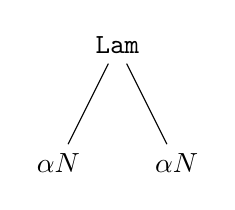
\begin{tikzpicture}
    \begin{scope}[every node/.style={font=\ttfamily}]
    \node (lam) {Lam}
    child {node (var) {$\Binder{\alpha}{\mathbb{N}}$}}
    child {node (var) {$\Var{\alpha}{\mathbb{N}}$}};
    \end{scope}
  \end{tikzpicture}
\end{center}

This syntactic distinction is important because it keeps the typing rules syntax directed, and \textsf{FParam}s and \textsf{AST}s need to have different types. If the type system did not distinguish \textsf{FParam}s and \textsf{AST}s, the following malformed AST would be well-typed:
\begin{center}
  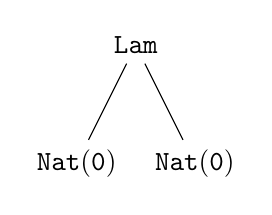
\begin{tikzpicture}
    \begin{scope}[every node/.style={font=\ttfamily}]
    \node (lam) {Lam}
    child {node (var) {Nat$($0$)$}}
    child {node (var) {Nat$($0$)$}};
    \end{scope}
  \end{tikzpicture}
\end{center}
% \item \textbf{\texttt{binderToAST}}, a primitive for turning binders (\underline{\texttt{Var}}) into \textit{usages} of binders (\texttt{Var})

% This allows for programs like the following:
% \begin{core}
% $\begin{array}{l}
%   \textbf{\texttt{do}} \, \, {x} \leftarrow {\Binder{\alpha}{\mathbb{N}}} \, \, \textbf{\texttt{in}} \\
%   \textbf{\texttt{do}} \, \, {\texttt{body}} \leftarrow \textbf{\texttt{binderToAST}} \, x \, \, \textbf{\texttt{in}} \\
%   \textbf{\texttt{return}} \, \, \texttt{Lam}(x, \texttt{body})
% \end{array}$
% \vspace{2mm} 
% \textcolor{coreComment}{\hrule height 0.2mm \relax}
% \vspace{2mm} 

% \textcolor{coreComment}{$\begin{array}{l}\return{\texttt{Lam}(\Binder{\alpha}{\mathbb{N}}, \Var{\alpha}{\mathbb{N}})}\end{array}$}
% \end{core}

\item $\gensym{R}$, a primitive for generating fresh formal parameters of type $R$, $\Binder{\alpha}{R}$, where two different calls to \textbf{\texttt{mkvar}} should return two different formal parameters.

The need for \textbf{\texttt{mkvar}} arises from treating \coreLang{} as an elaboration target for \sourceLang{}. Consider \Cref{listing:source-gensym}, which should generate the AST of $\lambda \alpha. \lambda \beta. \, \return{(\alpha, \beta)}$.

\begin{minipage}[t]{\linewidth}
\begin{sourcelst}
$\begin{array}{l}
\$(\textbf{\texttt{do}} \, \, \texttt{mkfun} \leftarrow {\lambda k. \, {\langle\langle\,\, \lambda x: \mathbb{N}^0. \,\, \splice[(k \, {\equote[x]})]\,\, \rangle\rangle}} \, \, \textbf{\texttt{in}} \\
\quad \texttt{mkfun} \,\, (\,\, \lambda a. \, \texttt{mkfun} \, (\lambda b. \, \return{(a, b)})) \,\, )
\end{array}$

\vspace{2mm} 
\textcolor{sourceComment}{\hrule height 0.2mm \relax}
\vspace{2mm} 

\textcolor{sourceComment}{$\begin{array}{l}\return{\texttt{Lam}(\Binder{\alpha}{\mathbb{N}}, \texttt{Lam}(\Binder{\beta}{\mathbb{N}}, \texttt{Ret}(\texttt{Pair}(\Var{\alpha}{\mathbb{N}}, \Var{\beta}{\mathbb{N}}))))}\end{array}$}
\end{sourcelst}
\captionof{listing}{An example \sourceLang{} program which illustrates the need for \textbf{\texttt{mkvar}}}%
\label{listing:source-gensym}
\end{minipage}
\par\vspace{0.6\baselineskip}
The compile-time function \texttt{mkfun} (\citeauthor{taha-1999}'s \citep{taha-1999} \texttt{back}) is a higher-order function that accepts some compile-time function $k$. \texttt{mkfun} creates a binder ($\lambda x. \_$) and passes the formal parameter $x$ to $k$. $k$ uses $x$ to construct the \textsf{body} of a function $\lambda x. \textsf{body}$. For example, $\texttt{mkfun} \,  (\lambda y. \equote[{\splice[(y)]} + \texttt{1}])$ generates the body $x + \texttt{1}$.

In \Cref{listing:source-gensym}, $k$ calls \texttt{mkfun}. This constructs a \textit{nested} function, whose formal parameters are bound to $a$ and $b$ respectively. If $x$ was not renamed, and simply elaborated into $\Binder{x}{\mathbb{N}}$, both $a$ and $b$ would be bound to $\Binder{x}{\mathbb{N}}$, generating the following (incorrect) AST: 
 \[\return{\texttt{Lam}(\Binder{x}{\mathbb{N}}, \texttt{Lam}(\Binder{x}{\mathbb{N}}, \texttt{Ret}(\texttt{Pair}(\Var{x}{\mathbb{N}}, \Var{x}{\mathbb{N}}))))}\]
 Thus, \texttt{mkfun} should be elaborated into a function that generates \textit{fresh} names for $x$ each time it is called. This is the purpose of \textbf{\texttt{mkvar}}. 
\end{enumerate}

Second, \coreLang{} extends \efflang{} with machinery for scope extrusion checking. This machinery comprises:
\begin{enumerate}
\item \err{}, an error state for indicating the presence of scope extrusion,
\item \textbf{\texttt{check}}, a guarded \textbf{\texttt{return}} that either detects scope extrusion, and transitions to \textbf{\texttt{err}}, or does not detect scope extrusion, and transitions to \textbf{\texttt{return}},
\item \textbf{\texttt{check$_M$}}, which behaves similarly to \textbf{\texttt{check}}, but (as \Cref{section:best-effort-check} explains) allows a set of \textit{muted} variables $M$ to \textit{temporarily} extrude their scope,
\item \textbf{\texttt{dlet}}, a primitive for tracking which variables are well-scoped and which have extruded their scope,
\item \textbf{\texttt{tls}}, a marker representing an occurrence of a top-level splice in the source program. 
\end{enumerate}

\begin{figure}
\begin{core-desc}
  {\large \textbf{Syntax}} \\

  $\begin{array}{@{}llll}
    \textbf{Formal Parameters} & \alpha_R \\
    \textbf{Normal Forms} & n & ::= & \text{the natural lifting of \efflang{} values} \\
    &&& \mid  \Nat{m} \mid \alpha_R \mid \Var{\alpha}{R} \mid \Lam{n_1}{n_2}  \\ 
  &&&\mid \App{n_1}{n_2} \mid \Continue{n_1}{n_2} \mid \Ret{n}   \\ 
  &&& \mid \Do{n_1}{n_2}{n_3} \mid \Op{n} \mid \Hwith{n_1}{n_2}   \\
  &&&\mid \Hret{n_1}{n_2}(n_1, n_2) \mid \Hop{n_1}{n_2}{n_3}{n_4} \\
  \textbf{Terms} & t & := & \text{the natural lifting of \efflang{} computations} \\
  &&& \mid \checkfv{n} \mid \checkm{n} \mid \dlet{n}{t} \mid \tls{t} \mid \err \\
  \textbf{Handlers} & h & := & \text{the natural lifting of \efflang{} handlers} \\
  \end{array}$
\end{core-desc}
\caption{\coreLang{} syntax. The syntax extends \efflang{} with a (countably finite) class of (type-annotated) formal parameters, AST constructors and scope extrusion checking machinery.}
\label{fig:core-syntax}
\end{figure}

Notice that, while the calculus provides the \textit{machinery} for scope extrusion checking, it does not demand that one \textit{use} it, or use it \textit{properly}. Scope extrusion checking is not a language feature, but an algorithm one builds on top of the calculus. 
\subsection{Operational Semantics}
The semantics of \coreLang{} are made precise via an operational semantics. Many rules are identical to those of \efflang{} (\Cref{fig:efflang-opsem}): interesting rules are collated in \Cref{fig:corelang-opsem}. Rules are divided into those related to AST construction (\textsc{Ast-Rule}), and those related to \textbf{s}cope \textbf{e}xtrusion \textbf{c}hecking (\textsc{Sec-Rule}).

\newcommand{\coreConfiguration}[5]{\langle {#1}; {#2}; {#3}; {#4}; {#5} \rangle}
  % \renewcommand{\transition}[2]{#1 & \rightarrow & #2}
  % \renewcommand{\rulename}[2]{(\textsc{{#1}-{#2}})}
  \newcommand{\astRule}[1]{\rulename{Ast}{#1}}
  \newcommand{\secRule}[1]{\rulename{Sec}{#1}}
  % \newcommand{\effectRule}[1]{\rulename{Eff}{#1}}

\begin{figure}[t]
\begin{core-desc}
  \large{\textbf{Operational Semantics}}\\
  \normalsize{\textit{Selected Rules}}\\

  {
    \scriptsize

{\textbf{Evaluation Contexts}}\\
\[F ::= \ldots \mid \dlet{\Binder{\alpha}{R}}{[-]} \mid \tls{[-]} \] 
 {\textbf{Operational Semantics}}\\
\[
  \begin{array}{@{}rrcl}
  \astRule{Gen} & \transition{\coreConfiguration{\gensym{R}}{E}{U}{M}{I}}{\coreConfiguration{\return{\Binder{\alpha}{R}}}{E}{U\cup\{\alpha\}}{M}{I}}\\
  &&&\text{(where $\alpha = \textsf{next}(U), \; \textsf{next}(U) \notin U, \; \text{\textsf{next} deterministic}$)}\\
  \vspace{1mm}
  \\ 
  \secRule{Chs} & \transition{\coreConfiguration{\checkfv{n}}{E}{U}{M}{I}}{\coreConfiguration{\return{n}}{E}{U}{M}{I}}\\
    &&&\text{(if $\freevars{n} \subseteq \projfvs{E}$)}\\
  \secRule{Chf} & \transition{\coreConfiguration{\checkfv{n}}{E}{U}{M}{I}}{\coreConfiguration{\err}{E}{U}{M}{I}}\\
  &&&\text{(if $\freevars{n} \not\subseteq \projfvs{E}$)}       \\\vspace{1mm}\\
  \secRule{Cms} & \transition{\coreConfiguration{\checkm{n}}{E}{U}{M}{I}}{\coreConfiguration{\return{n}}{E}{U}{M}{I}}\\
    &&&\text{(if $\freevars{n} \setminus M \subseteq \projfvs{E}$)}\\
  \secRule{Cmf} & \transition{\coreConfiguration{\checkm{n}}{E}{U}{M}{I}}{\coreConfiguration{\err}{E}{U}{M}{I}}\\
  &&&\text{(if $\freevars{n} \setminus M \not\subseteq \projfvs{E}$)}
\\ 
 \vspace{1mm}
\\
\secRule{Tls} & \transition{\coreConfiguration{\tls{\return{n}}}{E}{U}{M}{I}}{\coreConfiguration{\return{n}}{E}{U}{\textcolor{coreHighlight}{\emptyset}}{\textcolor{coreHighlight}{\top}}}\\\vspace{1mm}
\\
  \secRule{Dlt} & \transition{\coreConfiguration{\dlet{\Binder{\alpha}{R}}{\return{n}}}{E}{U}{M}{I}}{\coreConfiguration{\return{n}}{E}{U}{\textcolor{coreHighlight}{M'}}{\textcolor{coreHighlight}{I'}}}\\
   &&&\text{\textcolor{coreHighlight}{(if $\textsf{len}(E) > I$ then $M' = M, I' = I$}}\\
   &&&\text{\textcolor{coreHighlight}{else $M' = \emptyset, I' = \top$)}}\\
   \effectRule{Op} & \transition{\coreConfiguration{\op{v}}{E_1[\handleWith{E_2}{h}]}{U}{M}{I}}\coreConfiguration{c[v/x, \text{cont}/ k]}{E_1}{U}{\textcolor{coreHighlight}{M \cup \projfvs{E_2}}}{\textcolor{coreHighlight}{I'}}\\
  &&& \text{(where cont $=\kappa x. \, \handleWith{E_2[\return{x}]}{h}$}\\
  &&& \text{and $\opHandler{x}{k}{c} \in h$ and $\textbf{\textsf{op}} \notin \textsf{handled}(E_2)$}\\
  &&& \text{and \textcolor{coreHighlight}{$I' = \textsf{min}(\textsf{len}(E_1), I)$})}
  \end{array} \]
  }
\end{core-desc}
\caption{Selected rules of the \coreLang{} operational semantics. Many of the rules can be trivially adapted from the \efflang{} semantics (\Cref{fig:efflang-opsem}). The muting and unmuting of variables is complex, and explained in \Cref{section:best-effort-check}. For now, these mechanisms are \textbf{\textcolor{coreHighlight}{highlighted}}.}%
\label{fig:corelang-opsem}
\end{figure}

\subsubsection{Configurations}
Like \efflang{}, the operational semantics is defined over \textit{configurations}. In \coreLang{}, configurations have the form:
\[\langle t; E; U; M; I \rangle\]
At a high level, $t$ and $E$ are terms and evaluation contexts respectively. $U$ acts as a source of freshness for name generation. $M$ is a set of muted variables, i.e. those that do not trigger a scope extrusion error, even if they have extruded their scope. $I$ indicates the point at which variables in $M$ should be \textit{unmuted}, by setting $M$ to $\emptyset$. 

\subsubsection{AST Rule}
The \textsc{Ast-Gen} rule describes the behaviour of \textbf{\texttt{mkvar}}: $\gensym{R}$ produces a formal parameter of type $R$ and some name $\alpha$. Recall that names should be \textbf{fresh}: that is, multiple calls to \textbf{\texttt{mkvar}} should always return variables with different names. This involves remembering names that have been previously generated, which are collected in $U$. To ensure determinacy of the semantics, names are chosen \textit{deterministically}.

% The other primitive, \textbf{\texttt{binderToAST}}, turns binders $\Binder{\alpha}{R}$ into usages of the binder $\Var{\alpha}{R}$ (\textsc{Ast-Use}). 

\subsubsection{Scope Extrusion Checking Rules}
The \textbf{\texttt{check}} primitive acts like a guarded \textbf{\texttt{return}}, which can catch occurrences of scope extrusion. For some arbitrary normal form $n$ of AST type, either:
\begin{enumerate}
  \item All the free variables of $n$ are properly scoped, so $\checkfv{n}$ reduces to $\return{n}$ (\textsc{Sec-Chs})
  \item Some free variables of $n$ are not properly scoped, so $\checkfv{n}$ reduces to $\err$ (\textsc{Sec-Chf})
\end{enumerate}
What does it mean to be ``properly scoped'' (the side condition on \textsc{Sec-Chs})? The answer is slightly subtle. Consider the following program 
\[\bind{\texttt{body}}{\checkfv{\Var{\alpha}{\mathbb{N}}}}{\checkfv{\Lam{\Binder{\alpha}{\mathbb{N}}}{\texttt{body}}}}\]
$\Var{\alpha}{\mathbb{N}}$ should be ``properly scoped'': it should not cause a transition to $\err$. However, it is hard to deduce this from the \textit{static} structure of the program. Instead, one has to reason about the \textit{dynamic} execution of the program. Rather than calculating what is properly scoped as a \textit{language feature}, \coreLang{} defers it to the programmer. Following \citet{kiselyov-2024}, the programmer must \textit{declare} that a variable is properly scoped through use of the \textbf{\texttt{dlet}} keyword. 
\[\dlet{\Binder{\alpha}{\mathbb{N}}}{\bind{\texttt{body}}{\checkfv{\Var{\alpha}{\mathbb{N}}}}{\checkfv{\Lam{\Binder{\alpha}{\mathbb{N}}}{\texttt{body}}}}}\]
More precisely, \textbf{\texttt{dlet}} places a frame of the form $\dlet{\Binder{\alpha}{R}}{[-]}$ on the evaluation context $E$. The notation $\projfvs{E}$ filters out the variables declared in this manner from $E$. For example,
\[\projfvs{\dlet{\Binder{\alpha}{R}}{\bind{x}{[-]}{t}}} = \{ \Var{\alpha}{R} \}\]

Given a term $E[t]$, I say variable $\Var{\alpha}{R}$ in $t$ is ``declared safe'' if $\Var{\alpha}{R} \in \projfvs{E}$ (\Cref{dfn:declared-safe}):
\begin{definition}[Declared Safe]{coreHighlight}\label[definition]{dfn:declared-safe}
  Given a term $E[t]$, $\Var{\alpha}{R}$ in $t$ is declared safe if $\Var{\alpha}{R} \in \projfvs{E}$
\end{definition}

Given a term of the form $\checkfv{n}$ in some evaluation context $E$, where $n$ is an AST, \textbf{\texttt{check}} thus succeeds if and only if the free \texttt{Var}s of $n$, written $\freevars{n}$, have all been declared safe, $\freevars{n} \subseteq \projfvs{E}$. 

It may seem lazy to define the semantics of \textbf{\texttt{check}} in such a way that places the burden onto the user. Recall, however, that \coreLang{} is \textit{not} meant to be programmed in directly. Rather, it acts as an elaboration target for \sourceLang{}. Therefore, the onus is on the person defining the elaboration to justify that \textbf{\texttt{dlet}} and \textbf{\texttt{check}} are used appropriately. 

\textbf{\texttt{check}}$_M$ is a variant of \textbf{\texttt{check}}. As \Cref{section:best-effort-check} explains, to design an optimal scope extrusion check, it is helpful to \textit{mute} some variables, pretending that they are properly scoped. \textbf{\texttt{check}}$_M$ behaves exactly like \textbf{\texttt{check}}, except that it pretends that the muted variables $M$ are properly scoped ($\checkm{n}$ succeeds if $\freevars{n} \text{\colorbox{yellow}{$ \, \setminus \, M$}} \subseteq \projfvs{E}$).

Similarly, when justifying the correctness of scope extrusion checks, it is useful to remember the position of top-level splices in the \sourceLang{} source program. The \textbf{\texttt{tls}} marker indicates the occurrence of a top-level splice in the source program. Beyond unmuting variables (\Cref{section:best-effort-check}), \textbf{\texttt{tls}} has no operational behaviour (\textsc{Sec-Tls}).

The final two rules, \textsc{Sec-Dlt} and \textsc{Eff-Op}, mute or unmute \texttt{Var}s. Muting and unmuting are explained in \Cref{section:best-effort-check}. For now, the components of transitions corresponding to muting and unmuting are \textbf{\textcolor{coreHighlight}{highlighted}}, and can be ignored. 

Ignoring muting and unmuting, \textsc{Sec-Dlt} silently removes a $\dlet{\Binder{\alpha}{R}}{[-]}$ frame
\[\langle \dlet{\Binder{\alpha}{R}}{\return{n}}; \textcolor{comment}{E};\textcolor{comment}{U};\textcolor{comment}{M};\textcolor{comment}{I}\rangle \to \langle \return{n}; \textcolor{comment}{E};\textcolor{comment}{U};\textcolor{comment}{M'};\textcolor{comment}{I'}\rangle\]
and \textsc{Eff-Op} behaves as it does in \efflang{} (\Cref{fig:efflang-opsem}):
\[
\begin{array}{lll}
\transition{\coreConfiguration{\op{v}}{E_1[\handleWith{E_2}{h}]}{\textcolor{comment}{U}}{\textcolor{comment}{M}}{\textcolor{comment}{I}}}\coreConfiguration{c[v/x, \text{cont}/ k]}{E_1}{\textcolor{comment}{U}}{\textcolor{comment}{M \cup \projfvs{E_2}}}{\textcolor{comment}{I'}}\\
  && \text{\footnotesize (cont $=\kappa x. \, \handleWith{E_2[\return{x}]}{h}$,}\\
  && \text{\footnotesize \,\,\,$\opHandler{x}{k}{c} \in h$ and $\textbf{\textsf{op}} \notin \textsf{handled}(E_2)$)}\\
\end{array}\]
% At a high level, when an operation is performed, we mute some set of variables, and potentially update the point at which they should be unmuted. When we remove a declared variable, we additionally check if we ought to unmute variables (and do so if we should).

\subsection{Type System}
\coreLang{} extends \efflang{} types with an \textsf{FParam} type and an \textsf{AST} type (\Cref{fig:core-types}).

\begin{figure}[t]
  \begin{core-desc}
    {\large {\textbf{Types}}}\\
    \textit{Computation and Handler Types omitted}\\

    \textbf{Run-time Pre-types}\\
    $\begin{array}{@{}lllr}
    \text{Effects Row} & \xi ::= \emptyset \mid \xi \cup \{ \texttt{op}_i \} \\
    \\
    \text{Value type} & Q,R ::= \mathbb{N} & \\
                              &\quad\quad\quad\,\, \mid \functionType[\xi]{Q}{R} & \text{functions}\\
                              &\quad\quad\quad\,\, \mid \continuationType[\xi]{Q}{R} & \text{continuations}\\ \\
    \text{Computation type} & \effectType[\xi]{R} \\
    \text{Handler type} & \handlerType{\effectType[\xi_1]{Q}}{\effectType[\xi_2]{R}}
    \end{array}$
    
    \vspace{4mm}

    \textbf{Types}\\
  $\begin{array}{@{}lllr}
    % \text{Effects Row} & \Delta ::= \emptyset \mid \Delta \cup \{ \texttt{op}_i \} \\
    % \\
    % \text{}
    \text{Value type} & S, T ::= \ldots\\
                              &\quad\quad\quad\,\, \mid \textsf{FParam}(R) & \text{formal parameter}\\
                              &\quad\quad\quad\,\, \mid \textsf{AST}(R) & \text{AST (value)}\\
                              &\quad\quad\quad\,\, \mid \textsf{AST}(\effectType[\xi]{R}) & \text{AST (computation)}\\
                              &\quad\quad\quad\,\, \mid \textsf{AST}(\handlerType{\effectType[\xi_1]{Q}}{\effectType[\xi_2]{R}}) & \text{AST (handler)}\\
    % \text{Computation type} & \effectType{T} \\
    % \text{Handler type} & \handlerType{\effectType{S}}{\effectType[\Delta_2]{T}}
  \end{array}$
  \end{core-desc}
  \caption{The types of \coreLang{}. \coreLang{} types extend \efflang{} types with an \textsf{AST} type (for ASTs), and an \textsf{FParam} type}%
  \label{fig:core-types}
\end{figure}

% The role of the \textsf{AST} type is clear, but the role of \textsf{FParam} less so. I illustrate the purpose of the \textsf{FParam} type by example. Consider the following malformed AST:

% \begin{center}
%   \begin{tikzpicture}
%     \begin{scope}[every node/.style={font=\ttfamily}]
%     \node (lam) {Lam}
%     child {node (var) {Nat($0$)}}
%     child {node (var) {Nat($0$)}};
%     \end{scope}
%   \end{tikzpicture}
% \end{center}

% The aforementioned malformed AST should be ill-typed. To do so, it is insufficient to require that the left sub-tree is of type $\textsf{AST($\mathbb{N}$)}$. It must specifically be a \underline{\textsf{Var}} AST node. That is the purpose of the \textsf{FParam} type. 

\subsubsection{Typing Rules}
The \coreLang{} typing rules (\Cref{fig:core-typing-rules}) are extremely straightforward: for example, $\Binder{\alpha}{R}$ is an \textsf{FParam} of type $R$, and $\Var{\alpha}{R}$ is an \textsf{AST} of type $R$. $\gensym{R}$ is a computation that produces \textsf{FParam}s of type $R$, and $\Lam{n_1}{n_2}$ is well-typed if $n_1$ is an \textsf{FParam} and $n_2$ an AST. 

Notice that this type system does not guarantee that the resulting AST is \textit{well-scoped}, for example, the following is well-typed:
\[\cdot \vdash {\Var{\alpha}{R}}: {\textsf{AST}(R)}\]

The typing rules for scope extrusion checks are even more straightforward: they are effectively invisible to the type system. The only complex case is \textbf{\texttt{err}}, which can be assigned any type in any context. \textbf{\texttt{err}} thus behaves similarly to \textbf{\texttt{absurd}} in \texttt{Haskell}, or in the $\lambda$-calculus extended with the empty type \citep{scherer-2017}.

A closed \coreLang{} term is well-typed if it can be typed with an empty effects row. 
\begin{definition}[Well-typed closed term]{coreHighlight}
A closed term $t$ is well-typed if $\cdot \vdash t: T \, ! \,  \emptyset$
\end{definition}
\begin{figure}
  \begin{core-desc}
    {\large \textbf{Typing Rules}}\\
    \textit{Selected Rules}
    \begin{center} 
    \begin{minipage}[t]{0.32\textwidth}
      \centering
    $\inferrule[(Binder)]{ \\ }{\type{\Binder{\alpha}{R}}{\textsf{FParam}(R)}}$
    \end{minipage}%
    \begin{minipage}[t]{0.32\textwidth}
      \centering
    $\inferrule[(Variable)]{ \type{n}{\textsf{FParam}(R)} }{\type{\varToAST{n}}{\textsf{AST}(R)}}$
    \end{minipage}%
    \begin{minipage}[t]{0.36\textwidth}
      \centering
    $\inferrule[(Mkvar)]{ \\ }{\type{\gensym{R}}{\effectType{\textsf{FParam}(R)}}}$
    \end{minipage}

      \vspace{5mm}

    \begin{minipage}[t]{\textwidth}
      \centering
    $\inferrule[(Lambda-AST)]{\type{n_1}{\textsf{FParam}(Q)}\\{\type{n_2}{\textsf{AST}(\effectType[\xi]{R})}}}{\type{\Lam{n_1}{n_2}}{\textsf{AST}(\functionType[\xi]{Q}{R})}}$
    \end{minipage}

    \vspace{5mm}

    \begin{minipage}[t]{0.25\textwidth}
      \centering
    $\inferrule[(Err)]{    }{\type{\err}{\effectType{T}}}$
    \end{minipage}%
    \begin{minipage}[t]{0.25\textwidth}
      \centering
    $\inferrule[(Tls)]{\type{t}{\effectType{T}}}{\type{\tls{t}}{\effectType{T}}}$
    \end{minipage}%
    \begin{minipage}[t]{0.5\textwidth}
      \centering
    $\inferrule[(DLet)]{\type{n}{\textsf{FParam}(R)} \\ \type{t}{\effectType{T}}}{\type{\dlet{n}{t}}{\effectType{T}}}$
    \end{minipage}

    % \vspace{5mm}

    % \begin{minipage}[t]{\textwidth}
    %   \centering
    % $\inferrule[(BinderToAST)]{\type{n}{\textsf{FParam}(R)}}{\type{\varToAST{n}}{\textsf{AST}(R)}}$
    % \end{minipage}

    \vspace{5mm}

    \begin{minipage}[t]{\textwidth}
      \centering
    $\inferrule[(Check)]{\type{n}{T} \\ T = \textsf{AST}(R) \lor \textsf{AST}(\effectType[\xi]{R}) \lor \textsf{AST}(\handlerType{\effectType[\xi_1]{Q}}{\effectType[\xi_2]{R}})}{\type{\checkfv{n}}{\effectType{T}}}$
    \end{minipage}

  \end{center}
  \end{core-desc}

\caption{Selected \coreLang{} typing rules}
\label{fig:core-typing-rules}
\end{figure}
 
\subsection{Implementation}
The core calculus \coreLang{} corresponds to a concrete \texttt{OCaml} implementation. In the concrete \texttt{OCaml} implementation, \textbf{\texttt{check}}, \textbf{\texttt{dlet}}, and \textbf{\texttt{err}} are not primitives. Rather, they are encoded as a \textit{mode of use} of effects and handlers. 
\begin{enumerate}
  \item $\checkfv{n}$ is implemented by performing a \texttt{FreeVar} effect, that are passed the free variables of $n$\\ 
  $\checkm{n}$ is similar, except there are also \texttt{Mute} and \texttt{Unmute} effects
  
  \item $\dlet{\Binder{\alpha}{R}}{t}$ is implemented as a \textit{handler} of the \texttt{FreeVar} effect, which subtracts $\Var{\alpha}{R}$ from the set of free variables, and either:
  \begin{enumerate}
    \item Resumes the continuation, if the set of free variables is now empty (all free variables declared safe)
    \item Performs another \texttt{FreeVar} effect, to check that the remaining free variables are declared safe. Following a successful such check, the continuation may be resumed.
  \end{enumerate}
  \item \textbf{\texttt{err}} is an unhandled \texttt{FreeVar} effect
\end{enumerate}

\section{Elaboration from \texorpdfstring{\sourceLang{}}{Lambda-Op-Quote-Splice} to \texorpdfstring{\coreLang{}}{Lambda-Op-AST}}\label{section:elaboration}
This section describes an elaboration from \sourceLang{} to \coreLang{}. This elaboration is simple: it does not insert any dynamic scope extrusion checks (other elaborations in \Cref{chapter:scope-extrusion}, that do insert checks, are built by extending this elaboration).

\newcommand{\elaborate}[1]{\llbracket #1 \rrbracket}
\newcommand{\erase}[1]{\textsf{erase}(#1)}
\newcommand{\AST}[1]{\textsf{AST}(#1)}
\newcommand{\Code}[1]{\textsf{Code}(#1)}


The elaboration is defined on typing judgements: \sourceLang{} judgements elaborate to \coreLang{} judgements. This decomposes into four elaborations: on effect rows, types, contexts, and terms. As the specific elaboration is clear from the context, I write $\llbracket - \rrbracket$ for all four.

\subsection{Elaborating Effect Rows}
Elaborating effect rows is just the identity, that is 
\[\begin{array}{rcl}
  \elaborate{\Delta} &=& \Delta \\
  \elaborate{\xi}&=&{\xi}
\end{array}\]

\subsection{Elaborating Types}
To define the elaboration of types, it is convenient to refer to a helper function, \textsf{erase} (\Cref{appendix:auxiliary-erase}), that, given a level $0$ type, \textit{erases} all of the level annotations (and elaborates effect rows), producing a run-time pre-type. For example: 
\[\textsf{erase}((\functionType[\xi]{S^0}{T^0})^0) = \functionType[\elaborate{\xi}]{S}{T}\]
In a nutshell, level $0$ types elaborate into \textsf{AST} types, and level $-1$ types elaborate into themselves (sans level annotations), except for \textsf{Code} types, which elaborate into \textsf{AST} types ($\elaborate{\textsf{Code}(\effectType{T^0})^{-1}} = \elaborate{\effectType{T^0}}$).
\[
\begin{array}{rcl}
  \elaborate{T^0} & = & \AST{\erase{T^0}}\\
  \elaborate{\effectType[\xi]{T^0}} & = & \AST{\erase{\effectType[\xi]{T^0}}}\\
  \elaborate{\effectType[\Delta]{T^0}} & = & \effectType[\elaborate{\Delta}]{\AST{\erase{T^0}}}\\
  \elaborate{\effectType[\Delta ; \xi]{T^0}} & = & \effectType[\elaborate{\Delta}]{\AST{\erase{\effectType[\xi]{T^0}}}}\\
  \elaborate{{(\handlerType{\effectType[\xi_1]{S^0}}{\effectType[\xi_2]{T^0}})}^0} & = & {\AST{\erase{(\handlerType{\effectType[\xi_1]{S^0}}{\effectType[\xi_2]{T^0}})^0}}}\\\\
  \elaborate{\mathbb{N}^{-1}} & = & \mathbb{N} \\
  \elaborate{(\functionType{S^{-1}}{T^{-1}})^{-1}} & = & \functionType[\elaborate{\Delta}]{\elaborate{S^{-1}}}{\elaborate{T^{-1}}} \\
  \elaborate{(\continuationType{S^{-1}}{T^{-1}})^{-1}} & = & \continuationType[\elaborate{\Delta}]{\elaborate{S^{-1}}}{\elaborate{T^{-1}}} \\
  \elaborate{\textsf{Code}({\effectType[\xi]{T^{0}}})^{{-1}}} & = & {\textsf{AST}(\erase{{\effectType[\xi]{T^{0}}}})}\\[2mm]
  \elaborate{\effectType{T^{-1}}} & = & \effectType[\elaborate{\Delta}]{\elaborate{T^{-1}}}\\[2mm]
  \elaborate{(\handlerType{\effectType[\Delta_1]{S^{-1}}}{\effectType[\Delta_2]{T^{-1}}})^{-1}} & = & \handlerType{\effectType[\elaborate{\Delta_1}]{\elaborate{S^{-1}}}}{\effectType[\elaborate{\Delta_2}]{\elaborate{T^{-1}}}}\\
  % \text{if} \, T \neq \Code{\effectType[\xi]{T^0}} \, \text{then} \, \erase{T^{-1}} \\ && \text{else}\, \AST{\erase{\effectType[\xi]{T^0}}}\\
  % \elaborate{\effectType{T^{-1}}} & = & \effectType[\elaborate{\Delta}]{\elaborate{T^{-1}}}\\
  % \elaborate{{(\handlerType{\effectType[\Delta_1]{S}}{\effectType[\Delta_2]{T}})}^{-1}} & = & {\erase{(\handlerType{\effectType[\Delta_1]{S}}{\effectType[\Delta_2]{T}})^{-1}}}
\end{array}
\]
\subsection{Elaborating Contexts}
Elaboration of contexts is subtle. Level $0$ types in the context are elaborated into \textsf{FParam}, rather than \textsf{AST} types. Elaboration of contexts thus requires a separate elaboration for context entries, and cannot rely naïvely on the elaboration on types.
\[
\begin{array}{rcl}
  \elaborate{\cdot} & = & \cdot \\
  \elaborate{\Gamma, x:T^0} & = & \elaborate{\Gamma}, x: \textsf{FParam}(\erase{T^0})\\
  \elaborate{\Gamma, x:T^{-1}} & = & \elaborate{\Gamma}, x: \elaborate{T^{-1}}
\end{array}
\]
To see why level $0$ types are elaborated into \textsf{FParam} types, notice that the only cases where the context $\Gamma$ is extended with a level $0$ variable occur in \compilemode{} or \quotemode{}. These modes build ASTs, and thus $x$ must be an \textsf{FParam}. 
% \subsection{Elaborating Effects}

\subsection{Elaborating Terms}
Elaboration of terms assumes that all formal parameters have been annotated with their types, for example: 
\[\lambda x: \mathbb{N}^0. \; e\]
The elaboration for terms is moderated by the \textbf{mode}: \compilemode{}, \quotemode{}, or \splicemode{}. Selected rules are collated in \Cref{fig:term-elaboration}. 

At a high level, in \compilemode{} and \quotemode{}-mode, one builds ASTs. To ensure formal parameters are appropriately renamed (\Cref{listing:source-gensym}), the elaboration must use \textbf{\texttt{mkvar}}. 

Take, for example, the elaboration of $\lambda x: {\mathbb{N}}^0. \; \return{x}$ in \compilemode{} or \quotemode{}, where $\textsf{erase}(\mathbb{N}^0) = \mathbb{N}$:
\begin{center}
  \begin{tikzpicture}
    \node[align=left](example){$\begin{array}{@{}l}\bind{x}{\gensym{\mathbb{N}}}{}\\
    \bind{\texttt{body}}{(\bind{n}{\return{\texttt{Var}({x})}}{\return{\Ret{n}}})}{}\\
    {\return{\Lam{x}{\texttt{body}}}}\end{array}$};

    \begin{scope}[on background layer, font=\scriptsize\bfseries, text=comment, align=left]
    \draw[draw=comment, line width = 0.3mm] ($(example.north) + (-3.7cm, 0.6cm)$) circle[radius=1.4mm] node (annote-1) {\tiny{1}};
    \node[anchor = east, align=right] (annote-1-text) at ($(annote-1.west) + (0.1cm, -0.15cm)$) {Generate fresh \\ \textsf{FParam} for $x$} ;
    \draw[draw=comment, line width =0.3mm] ($(example.north) + (-3.2cm, -0.1cm)$) |- (annote-1.east);

    \draw[draw=comment, line width = 0.3mm] ($(example.west) + (-0.4cm, -0cm)$) circle[radius=1.4mm] node (annote-2) {\tiny{2}};
    \node[anchor = east, align=right] (annote-2-text) at ($(annote-2.west) + (0.1cm, -0.15cm)$) {Generate \\ function body} ;
    \draw[draw=comment, line width =0.3mm] (example.west) -- (annote-2.east);

    \draw[draw=comment, line width = 0.3mm] ($(example.north east) + (-4.8cm, 0cm)$) circle[radius=1.4mm] node (annote-3) {\tiny{3}};
    \node[anchor = north west, align=left] (annote-3-text) at ($(annote-3.east) + (-0.1cm, 0.27cm)$) {Convert $x$ from \textsf{FParam} \\ to \textsf{AST} type} ;
    \draw[draw=comment, line width =0.3mm] ($(example.north east) + (-5.3cm, -0.6cm)$) |- (annote-3.west);

    \draw[draw=comment, line width = 0.3mm] ($(example.south east) + (-8.5cm, -0.3cm)$) circle[radius=1.4mm] node (annote-4) {\tiny{4}};
    \node[anchor = north west, align=left] (annote-4-text) at ($(annote-4.east) + (-0.1cm, 0cm)$) {Return AST of function} ;
    \draw[draw=comment, line width =0.3mm]  ($(example.south east) + (-9cm, 0.18cm)$) |- (annote-4.west);

  \end{scope}
    \end{tikzpicture}
\end{center}

Elaboration in \compilemode{} and \quotemode{}-modes do not differ significantly, with the exception of the rule for splice, where in \compilemode{}-mode, \textbf{\texttt{tls}} is inserted, and in \quotemode{}-mode, it is not. The \compilemode{} and \quotemode{}-modes become important when building scope extrusion checks. Elaboration in \splicemode{}-mode is effectively the identity. 

\newcommand{\cqmode}{\compilemode{} \mid \quotemode{}}
\begin{figure}
  \begin{source-desc}
    {\large\textbf{Term Elaboration}}\\
    \textit{Selected Rules}

    {\footnotesize
    \[
    \begin{array}{@{}lll}
      \elaborate{x}_{\cqmode} & = & \texttt{Var}(x)\\
      \elaborate{\lambda x: T^0. \, e}_{\cqmode} & = & \bind{x}{\gensym{\erase{T^0}}}{\bind{\texttt{body}}{\elaborate{e}_{\cqmode}}{\return{\Lam{x}{\texttt{body}}}}}\\\\
      \elaborate{\splice}_{\compilemode{}} & = & \tls{\elaborate{e}_{\splicemode{}}}\\
      \elaborate{\splice}_{\quotemode{}} & = & {\elaborate{e}_{\splicemode{}}}
      \\\\
      \elaborate{x}_{\splicemode{}} & = & x\\
      \elaborate{\lambda x: T^0. \, e}_{\splicemode{}} & = & \lambda x. \elaborate{e}_{\splicemode{}}\\
      \elaborate{\equote}_{\splicemode{}} & = & \elaborate{e}_{\quotemode{}}
    \end{array}
    \]
    }
  \end{source-desc}
  \caption{Selected term elaboration rules from \sourceLang{} to \coreLang{}. Term elaboration is very similar to \citet{calcagno-2003}, adapted for compile-time generation with top-level splices, and modes rather than levels. Elaboration is moderated by the compiler mode. In \compilemode{} and \quotemode{}, elaboration builds ASTs. In \splicemode{}-mode, elaboration is effectively the identity. }%
  \label{fig:term-elaboration}
\end{figure}

\subsection{Elaborating Typing Judgements}\label{subsection:typing-judgement-elaboration}
Elaboration of typing judgements can now be defined compositionally. For example, take the typing judgement for lambdas in \compilemode{}-mode:
\[
{\inferrule{\ctypejudge[\Gamma, x: S]{e}{\runtimecomptype{T}{\Delta;\xi}}}{\ctypejudge{\lambda x.e}{\runtimecomptype{(\functionType[\xi]{S}{T})}{\Delta}}}}
\]
which is elaborated by applying the elaboration component-wise:
\newcommand{\typejudge}[3][\Gamma]{#1 \vdash #2 : #3}
\[
{\inferrule{\typejudge[\elaborate{\Gamma, x: S}]{\elaborate{e}_{\compilemode{}}}{\elaborate{\runtimecomptype{T}{\Delta;\xi}}}}{\typejudge[\elaborate{\Gamma}]{\elaborate{\lambda x.e}_{\compilemode{}}}{\elaborate{\runtimecomptype{(\functionType[\xi]{S}{T})}{\Delta}}}}}
\]
Letting $R = \erase{S}$, $Q = \erase{T}$, and $\elaborate{e}_{\compilemode{}} = t$, and applying the elaboration functions defined above, we obtain \Cref{derivation:elaborated}, which, assuming that the premise is valid typing derivation, corresponds to a valid \coreLang{} typing derivation.
\begin{typederivation}[H]
  \small
\[
{\inferrule{\typejudge[\elaborate{\Gamma}, x: \textsf{FParam}(Q)]{t}{\effectType{\AST{\effectType[\xi]{R}}}}}{\typejudge[\elaborate{\Gamma}]{\bind{x}{\gensym{\erase{T^0}}}{\bind{\texttt{body}}{t}{\return{\Lam{x}{\texttt{body}}}}}}{\effectType{\AST{\functionType[\xi]{Q}{R}}}}}}
\]
\caption{The elaborated derivation of $\ctypejudge{\lambda x. e}{\functionType[\xi]{S}{T}}$}
\label{derivation:elaborated}
\end{typederivation}

Do \sourceLang{} typing derivations always elaborate into \coreLang{} typing derivations? Yes, but the question begets a larger point: what properties can be claimed about the calculus as defined? What metatheoretic results may be established?
\section{Metatheory}\label{section:metatheory}
This section states and proves several metatheoretic results about \sourceLang{} and \coreLang{}. 

First, well-typed \sourceLang{} programs elaborate into well-typed \coreLang{} programs:

\begin{theorem}[Elaboration Preservation]{sourceHighlight}
  If $\Gamma \vdash_{\star} e: \tau$ then $\elaborate{\Gamma} \vdash \elaborate{e}_{\star}: \elaborate{\tau}$, where $\star = \compilemode{} \mid \quotemode{} \mid \splicemode{}$ and $\tau$ is a level $0$ or level $-1$ value, computation, or handler type. 
\end{theorem}

The proof is by induction on the typing rules, e.g.\ \Cref{derivation:elaborated} in \Cref{subsection:typing-judgement-elaboration}.  

Additionally, the core language \coreLang{} satisfies appropriate progress and preservation properties. 

\begin{theorem}[Progress]{coreHighlight} 
If $\cdot \vdash {E[t]}: {\effectType{T}}$ then for all $U, M, I$ either 
\begin{enumerate}
\item $t$ is of the form $\return{n}$ and $E = [-]$,
\item $t$ is of the form $\op{v}$ for some $\textsf{op} \in \Delta$, and $\texttt{op} \notin \textsf{handled}(E)$
\item $t$ is of the form $\err$
\item $\exists t', E', U', M', I'$ such that $\langle t; E; U; M; I \rangle \rightarrow \langle t';E';U';M';I'\rangle$
\end{enumerate}
\end{theorem}
Note the third clause, which may be used by the calculus to report scope extrusion. 

The proof of progress by induction over the typing derivation. Since \coreLang{} is built by extending \efflang{}, the proof need only consider the augmented typing rules, all of which are straightforward.

\begin{theorem}[Reduction Preservation]{coreHighlight}
If $\cdot \vdash E[t]: \effectType{T}$ and $\langle t; E; U; M; I \rangle \to \langle t'; E'; U'; M'; I' \rangle$ 
then $\cdot \vdash E'[t']: \effectType{T}$ 
\end{theorem}
The proof of reduction preservation proceeds by induction over the operational semantics. Once again, one need only consider the augmented rules, which are simple. 

As a corollary, we obtain a notion of type safety.

\begin{corollary}[Type Safety]{sourceHighlight}\label[corollary]{cor:core-type-safety}
  If $\ctypejudge[\cdot]{e}{T^0 \, ! \, \emptyset;\emptyset}$ then either
  \begin{enumerate}
    \item $\langle \elaborate{e}_{\compilemode{}}; [-]; \emptyset
    ; \emptyset; \top \rangle \to^{\omega}$,
    \item $\langle \elaborate{e}_{\compilemode{}}; [-]; \emptyset; \emptyset; \top \rangle \to^{*} \langle \err; E; U; M; I \rangle$ for some $E$, $U$, $M$, $I$, or 
    \item $\langle \elaborate{e}_{\compilemode{}}; [-]; \emptyset; \emptyset; \top \rangle \to^{*} \langle \return{n}; [-]; U; M; I \rangle$ for some $U$, $M$, $I$
  \end{enumerate} 
where the initial configuration comprises an elaborated term, the empty evaluation context, an empty set indicating that no variables have been previously generated, another empty set indicating no variables have been muted, and $\top$, indicating that there is (currently) no plan to unmute variables.
\end{corollary}

Importantly, this notion of type safety is weak. A semantics which always reports a scope extrusion error (\textbf{\texttt{err}}) would be type safe under this definition. Further, a semantics which never reports scope extrusion would be type safe as well. Due to the potential presence of scope extrusion, the third case of \Cref{cor:core-type-safety} cannot additionally claim that the normal form $n$ represents a well-typed \efflang{} program. 

% In addition to type safety, we can formulate an equational theory for \sourceLang{}. First, I prove that, underneath a top-level splice, splice and quotation are duals. Second, I prove that \sourceLang{} is a fine-grain CBV calculus. 

% To formulate this equational theory, we will need a notion of contextual equivalence in \coreLang{}. In turn, this demands a notion of equality between \textsf{AST}s of values, computations, and handlers. I will abuse notation and write $n_1 =_\textsf{AST} n_2$, to represent all three. The notion of equality I choose is syntactic equality up to $\alpha$-renaming. So, for example, 
% \renewcommand{\Var}[2]{\texttt{Var}(#1_{#2})}

% \begin{center}
% \begin{tikzpicture}
%       \node (equals) {$=_{\textsf{AST}}$};

%   \begin{scope}[every node/.style={font=\ttfamily}, shift={($(equals.west) + (-3cm, 0.7cm)$)}]
%     \node (lam) {Lam}
%     child {node (var) {$\Binder{\alpha}{\mathbb{N}}$}}
%     child {node (var) {$\Var{\alpha}{\mathbb{N}}$}};
%     \end{scope}


%   \begin{scope}[every node/.style={font=\ttfamily}, shift={($(equals.east) + (3cm, 0.7cm)$)}]
%     \node (lam) {Lam}
%     child {node (var) {$\Binder{\beta}{\mathbb{N}}$}}
%     child {node (var) {$\Var{\beta}{\mathbb{N}}$}};
%     \end{scope}
    
% \end{tikzpicture}
% \end{center}
% but, however, 
% \begin{center}
% \begin{tikzpicture}
%       \node (equals) {$\neq_{\textsf{AST}}$};

%   \begin{scope}[every node/.style={font=\ttfamily}, shift={($(equals.west) + (-3cm, 0.7cm)$)}]
%     \node (lam) {Plus}
%     child {node (var) {1}}
%     child {node (var) {2}};
%     \end{scope}


%   \begin{scope}[every node/.style={font=\ttfamily}, shift={($(equals.east) + (3cm, 0.7cm)$)}]
%     \node (lam) {Plus}
%     child {node (var) {2}}
%     child {node (var) {1}};
%     \end{scope}
    
% \end{tikzpicture}
% \end{center}
% Syntactic equality is, of course, not the only sensible notion of equality. One can also choose, for example, contextual equivalence with respect to the \efflang{} semantics. Nevertheless, armed with this notion of equality on \textsf{AST} types, it is easy to define a notion of contextual equivalence in \coreLang{}. First, define ground types 
% \[T_\textsf{Ground} \triangleq \mathbb{N} \mid \textsf{AST}(R) \mid \textsf{AST}(\effectType[\xi]{R}) \mid \textsf{AST}(\handlerType{\effectType[\xi]{Q}}{\effectType[\xi_2]{R}})\]
% and a notion of equality on each ground type ($=_{\textsf{Ground}}$), which is just numerical equality for $\mathbb{N}$ and $=_{\textsf{AST}}$ for AST types. Then,
% \begin{definition}[Contextual Equivalence]{coreHighlight}\label{dfn:ctx-equiv}
%   $t$ and $t'$ are contextually equivalent at context $\Gamma$ and type $\effectType{T}$, written $\Gamma \vdash t \contextequiv t': '\effectType{T}$ if 
%   \begin{enumerate}
%     \item $\type{c}{\effectType{T}}$ and $\type{c'}{\effectType{T}}$
%     \item For all $E$ such that $\cdot \vdash {E[c]}: {\effectType[\emptyset]{T_{\textsf{Ground}}}}$  and $\cdot \vdash {E[c']}: {\effectType[\emptyset]{T_{\textsf{Ground}}}}$, we have either 
%     \begin{enumerate}
%       \item $\langle t; E; []; \emptyset; \top \rangle \to^{\omega}$ and $\langle t'; E; []; \emptyset; \top \rangle \, \to^{\omega}$,
%       \item For some $E_1$, $M_1$, $U_1$, $I_1$, $E_2$, $M_2$, $U_2$, $I_2$\\ $\langle t; E; []; \emptyset; \top \rangle \to^{*} \langle \err; E_1; M_1; U_1; I_1 \rangle$, and \\
%       $\langle t'; E; []; \emptyset; \top \rangle \to^{*} \langle \err; E_2; M_2; U_2; I_2 \rangle$
%       \item For some $M_1$, $U_1$, $I_1$, $M_2$, $U_2$, $I_2$\\ $\langle t; E; []; \emptyset; \top \rangle \to^{*} \langle \return{n}; [-]; M_1; U_1; I_1 \rangle$, and \\
%       $\langle t'; E; []; \emptyset; \top \rangle \to^{*} \langle \return{m}; [-]; M_2; U_2; I_2 \rangle$, and \\ 
%       $n =_{\textsf{Ground}} m$ 
%     \end{enumerate}
%     %  \, {\effconfiguration{\return{v}}{[-]}} \iff \effconfiguration{c'}{E} \, \to^{*} \, \effconfiguration{\return{v}}{[-]}
%   \end{enumerate}
% \end{definition}

% We can now prove the equational theory of \sourceLang{}. 

Finally, underneath a top-level splice, quotation and splice are duals (\Cref{thm:quote-splice-duality})

\begin{theorem}[Quote-Splice Duality]{sourceHighlight}\label{thm:quote-splice-duality}
  Under a top-level splice, quotation and splice are duals
  \[\begin{array}{rcl}
\splice[{\equote}] & =_{\quotemode{}} & e \\
\equote[{\splice}] & =_{\splicemode{}} & e
\end{array}
\]
\end{theorem}
Where $=_{\star}$ means ``elaborates to contextually equivalent \coreLang{} programs in $\star$ mode''. Parameterising by the mode is necessary, since the mode affects the result of elaboration. It is possible to prove something stronger: they elaborate to the same \coreLang{} program (contextual equivalence follows from reflexivity). The proof of quote-splice duality is by inspection of the definition of elaboration, where:
\[\begin{array}{rcl}  
  \elaborate{\splice[{\equote}]}_{\quotemode{}} = t & \iff & \elaborate{e}_{\quotemode{}} = t\\
  \elaborate{\equote[{\splice}]}_{\splicemode{}} = t & \iff & \elaborate{e}_{\splicemode{}} = t
\end{array}
  \]

% To prove that \sourceLang{} is a fine-grain CBV calculus (\Cref{dfn:fine-grain-cbv}) is only slightly more involved.  

% [TODO]